\documentclass[article,A4,12pt]{llncs}
\usepackage[T1]{fontenc}
\usepackage{amsmath}
\usepackage{amssymb}
\usepackage{amsfonts}
\usepackage{mathrsfs, bm}

\usepackage{graphicx}
\usepackage{tabularx}
\usepackage{subfig}
\usepackage{epsf,times}
\usepackage{color}
\usepackage{wrapfig}
\usepackage{cases}
\usepackage{multicol}

\usepackage[T1]{fontenc}
%\newcommand{\tmname}[1]{\textsc{#1}}
%\newcommand{\tmop}[1]{\ensuremath{\operatorname{#1}}}
%\newcommand{\tmsamp}[1]{\textsf{#1}}
%\newcommand{\tmtextsc}[1]{{\scshape{#1}}}
%\newcommand{\tmtextsl}[1]{{\slshape{#1}}}
%\newcommand{\tmtexttt}[1]{{\ttfamily{#1}}}

\leftmargin=0.0cm
\oddsidemargin=0.5cm
\evensidemargin=0.5cm
\topmargin=0cm
\textwidth=16.0cm
%\textheight=21.5cm
\textheight=20.0cm
\pagestyle{plain}
\setlength{\columnsep}{20pt}

\def\m{\mathbf{m}}
\def\H{\mathbf{H}}
\def\E{\mathbf{E}}
\newcommand{\vepsi}{{\varepsilon}}
\def\hnorm#1#2{\vert\,#1\,\vert_{#2}}
\newcommand{\R}{{\mathbb R}}
\newcommand{\Sph}{{\mathbb S}}
\def\x{\mathbf{x}}
\def\hvec{\overline{\mathbf{h}}}
\def\evec{\overline{\mathbf{e}}}

\newcommand{ \etal}{\mbox{\emph{et al. }}}

\newcommand\vect[1]{\mbf{#1}}
\newcommand{\mbf}[1]{\mbox{\boldmath$#1$}} 
\newcommand{\RC}[1]{#1 $\times$ #1 $\times$ #1}
\def\um{$\mu$m}
\def\C{$^{\circ}\mathrm{C}$}

\newcommand{\Rmnum}[1]{\expandafter\@slowromancap\romannumeral #1@}

% DEFINITION OF CUSTOM FONT SIZE
\newcommand{\customfontA}{\fontsize{50}{55}\selectfont}
\newcommand{\customfontB}{\fontsize{14.4}{20}\selectfont}
\newcommand{\customfontC}{\fontsize{30}{35}\selectfont}

\DeclareMathAlphabet{\mathpzc}{OT1}{pzc}{m}{it}

\def\clovek#1{\noindent\bgroup\vbox{\noindent#1}\egroup\vskip1em}

% TO INPUT BACKGROUND IMAGE
\usepackage{eso-pic}
\newcommand\BackgroundPic{
\put(0,0){
\parbox[b][\paperheight]{\paperwidth}{
\vfill
\centering
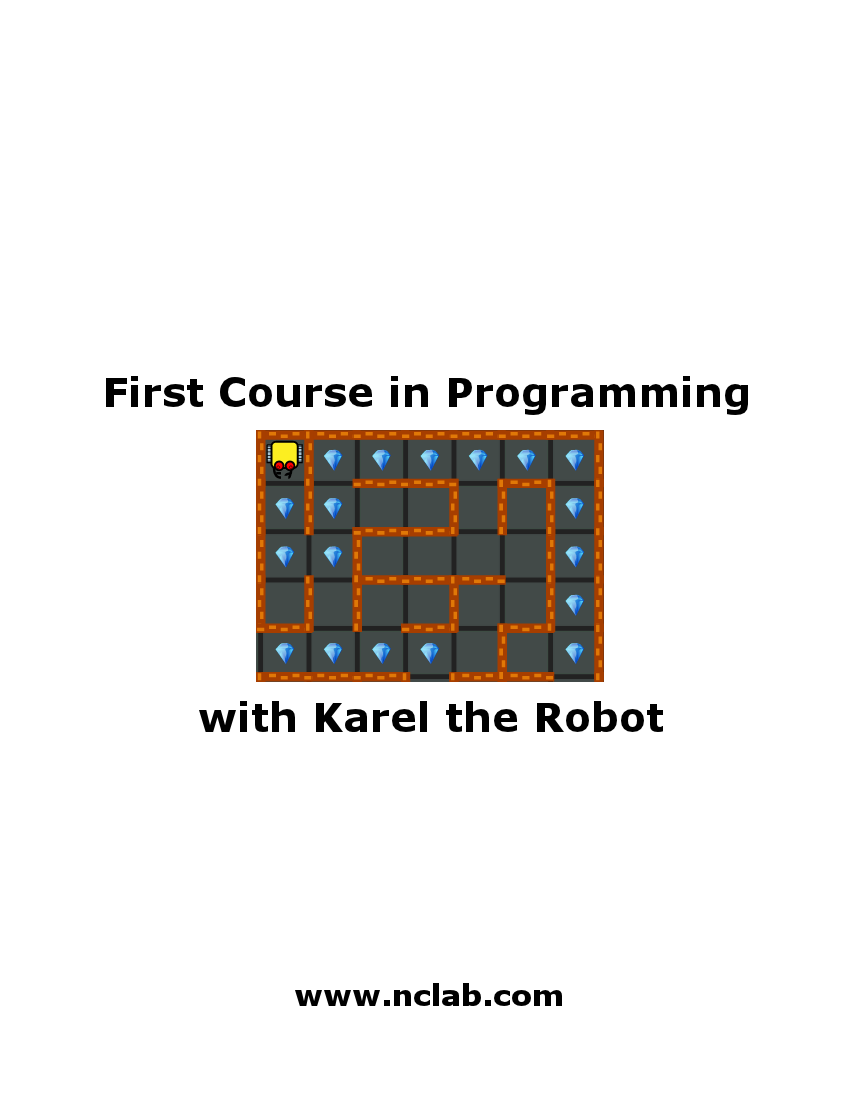
\includegraphics[width=\paperwidth,height=\paperheight]{img/karel-frontpage.png}
%\includegraphics[width=\paperwidth,height=\paperheight]{img/background.jpg}
\vfill
}}}

\begin{document}

% INPUTTING BACKGROUND IMAGE
\AddToShipoutPicture{\BackgroundPic}
\vbox{}
\pagestyle{empty}
\newpage
\textwidth=15.5cm
\ClearShipoutPicture
\newpage

%%%%%%%%%%%%%%%%%%%%%%%%%%%%%%%%%%%%%%%%%%%%%%%%%%%%%%%%%%%%%%%%%%%%%%%%%

\section*{}
\small
\input ../common/aboutnclab.tex

\subsection*{NCLab's Karel vs. the Original Version}
This publication features {\em Karel the Robot}, a programming language 
designed by Richard E. Pattis. Compared to the original version that
appeared in the 1980s and was strongly influenced by Pascal, the NCLab 
version is closer to Python.
There are some other differences as well that make Karel in NCLab easier to use 
for kids -- Karel collects gems instead of beepers, he has a home in the 
maze, and he uses commands that are much easier for kids to understand
and type. For example, {\tt pickbeeper} was replaced with {\tt get}, 
{\tt front-is-clear} was replaced with {\tt wall}, etc. We also introduced
a new command {\tt right} so that Karel acts more like a standard robot 
(in the original version of the language, where he only knew how to turn 
{\tt left}, he was swirling like a little tornado while solving more complex tasks).
Python colons following every command are omitted in the NCLab's version 
because using the SHIFT key was causing difficulties to 5 years old programmers. 
NCLab's Karel has a manual mode and three programming levels. Levels 1 and 2  
correspond to the Pattis' book. Level 3 brings a GPS device and the concept of 
variables. 

\normalsize

\newpage
%{\ }
\setcounter{tocdepth}{2}
\tableofcontents
%\pagestyle{plain}

\newpage

\pagestyle{plain}
\setcounter{page}{1}

%%%%%%%%%%%%%%%%%%%%%%%%%%%%%%%%%%%%%%%%%%%%%%%%%%%%%%%%%%%%%%%%%%%%%%%%%

\section{Introduction}

\subsection{Objectives} 

\begin{itemize}
\item Learn basic facts about the Karel language and its history. 
\item Learn how Karel differs from other programming languages.
\item Learn what this course will help you achieve.
\end{itemize}
This course will teach you principles of modern algorithmic design and  
computer programming with the help of an interactive graphical application 
{\em Karel the Robot} in NCLab. Taking this course will make it much easier 
for you to learn Python, C, C++ and other advanced programming languages. In particular we 
recommend that after Karel you continue with Python, a powerful programming 
language that is used across all science and engineering areas, and yet it is 
technically simpler to handle than C or C++. The textbook
{\em Python Programming for Beginners} is available in PDF via the link 
"Tutorials and Videos" on NCLab home page.

\subsection{Brief history}

Karel the Robot is a famous educational programming language that was introduced by Richard E. 
Pattis in his book "Karel The Robot: A Gentle Introduction to the Art of Programming" in 1981. 
Pattis first used the language in his courses at Stanford University, and now it is used at 
countless schools in the world to introduce students to algorithmic design and computer programming. 
The language is named after Karel \v{C}apek, a Czech writer who invented the word "robot" in his 1921 
science fiction play R.U.R. (Rossum's Universal Robots).

\subsection{Who is Karel?}

Karel is a little robot that lives in a maze, and there are gems in the maze that he loves to collect!
Sometimes multiple gems lie on each other, and in that case there is a number that shows their amount.
He was manufactured with only five simple commands in his memory:
\begin{itemize}
\item {\color{green} \tt go} ... make one step forward.
\item {\color{green} \tt get} ... pick up a gem from the ground. 
\item {\color{green} \tt left} ... turn to the left.
\item {\color{green} \tt right} ... turn to the right. 
\item {\color{green} \tt put} ... put a gem on the ground. 
\end{itemize}
He also has five built-in sensors that allow him to check his immediate surroundings:
\begin{itemize}
\item {\color{green} \tt wall} ... true if he would crash into a wall by making one more step, false otherwise. 
\item {\color{green} \tt gem} ... true if he stands on a gem, false otherwise.
\item {\color{green} \tt north} ... true if he is facing North, false otherwise.
\item {\color{green} \tt home} ... true if he is at home, false otherwise.
\item {\color{green} \tt empty} ... true if his bag with gems is empty, false otherwise. 
\end{itemize}
During this course you will help Karel solve many exciting tasks starting with very simple ones and 
gradually progressing to more challenging. In this way Karel becomes a great robot, and you 
will become a great programmer!

\subsection{Why should I take this course?}

Computer programming skills are highly valued today, and they will be even more 
valued in the future. Karel's language is so natural that you will be able to 
focus on designing great algorithms. This is the most important skill in 
computer programming. In other words, you could start learning programming 
with a technically 
complicated conventional programming language as well, but you would spend lots of time 
battling technical problems. The advantage of starting with Karel is that 
when moving on to other languages, you will be able to focus on the technical 
differences, as the programming concepts you will already understand.


\subsection{Is Karel a toy language?}

Definitely not! Despite its playful appearance, Karel contains all elements 
of modern procedural programming. The complexity of algorithms 
that you will encounter in this course ranges from {\em extremely simple} 
to {\em extremely tough}. Towards the end of this course you will encounter 
tasks that will make your head spin. However, Karel is very light on 
technicalities, which is very good for someone who is just starting out.

The biggest conceptual difference between Karel and standard procedural
programming languages such as Python, C, C++ or Fortran is that {\em the robot does not 
know math}. At least not until we get to advanced levels that are beyond 
the original Pattis' book. In the basic course, you will solve many exercises 
whose objective is to teach you how to design great algorithms, and math is 
not needed for that. After finishing this tutorial, you will be able to transition 
smoothly to Python where you can do as much math as you like!
 
\subsection{Review questions}

All review questions in this textbook are multiple-choice. One or more 
answers may be correct.

\begin{enumerate}
\item Name the university where Karel the Robot was created:
\begin{enumerate}
\item[A1] MIT
\item[A2] Princeton
\item[A3] Harvard
\item[A4] Stanford
\end{enumerate}
\item What is the programming language that you should learn after Karel?
\begin{enumerate}
\item[A1] C
\item[A2] Python
\item[A3] Haskell
\item[A4] Fortran
\end{enumerate}
\item What is the biggest conceptual difference between Karel and standard
      procedural programming languages such as Python, C, C++ or Fortran?
\begin{enumerate}
\item[A1] Karel only knows five commands.
\item[A2] Karel only can do simple algorithms.
\item[A3] Karel does not know math.
\item[A4] Karel has only five sensors.
\end{enumerate}
\item Where does Karel live and what objects does he like to collect?
\begin{enumerate}
\item[A1] Karel lives in a maze and he likes to collect gems.
\item[A2] Karel lives in a cave and he likes to collect gold nuggets.
\item[A3] Karel lives on an island and he likes to collect coconuts.
\item[A4] Karel lives in a marketplace and he likes to collect coins from the ground.
\end{enumerate}
\item What is the command that moves the robot one step forward?
\begin{enumerate}
\item[A1] step
\item[A2] forward
\item[A3] go
\item[A4] move
\end{enumerate}
\item What is the command that turns the robot to the left?
\begin{enumerate}
\item[A1] left\_turn
\item[A2] turn\_left
\item[A3] turnleft
\item[A4] left
\end{enumerate}
\item What is the command that turns the robot to the right?
\begin{enumerate}
\item[A1] right\_turn
\item[A2] right
\item[A3] turnright
\item[A4] turn\_right
\end{enumerate}
\item What is the command to pick up a gem from the ground?
\begin{enumerate}
\item[A1] pick
\item[A2] pick\_gem
\item[A3] get
\item[A4] get\_gem
\end{enumerate}
\item What is the command to drop a gem on the ground?
\begin{enumerate}
\item[A1] put
\item[A2] drop\_gem
\item[A3] drop 
\item[A4] put\_gem
\end{enumerate}
\item What sensor helps the robot avoid crashing into walls?
\begin{enumerate}
\item[A1] wall\_ahead
\item[A2] wall
\item[A3] crash
\item[A4] danger
\end{enumerate}
\item What sensor helps the robot detect gems?
\begin{enumerate}
\item[A1] detect\_gem
\item[A2] see\_gem
\item[A3] gem
\item[A4] near\_gem
\end{enumerate}
\item What sensor does the robot use to check whether he has any gems in his bag?
\begin{enumerate}
\item[A1] bag\_full
\item[A2] bag\_empty
\item[A3] has\_gems
\item[A4] empty
\end{enumerate}
\item What sensor helps the robot detect his orientation?
\begin{enumerate}
\item[A1] south
\item[A2] north
\item[A3] east
\item[A4] west
\end{enumerate}
\item What sensor helps the robot detect whether he is at home?
\begin{enumerate}
\item[A1] at\_home
\item[A2] finished
\item[A3] home
\item[A4] stop
\end{enumerate}
\item What is the most important skill in computer programming?
\begin{enumerate}
\item[A1] Writing short programs.
\item[A2] Designing great algorithms.
\item[A3] Writing programs quickly.
\item[A4] Knowing many programming languages.
\end{enumerate}
\end{enumerate}

%\section{Exploring NCLab}
%
%\subsection{Objectives} 
%
%\begin{itemize}
%\item Get acquainted with NCLab.
%\end{itemize}
%Before beginning this course, we invite you to create an account in 
%NCLab, log in, and take a while to explore the many activities 
%that NCLab offers. A great companion reading is {\em Intro to NCLab - Part I 
%(Meet the Cloud)} that is available in PDF via the link "Tutorials and Videos"
%on NCLab home page {\tt http://nclab.com}.
%
%\subsection{Review questions}
%
%Review questions for this Section are located in the document {\em Intro to NCLab - Part I 
%(Meet the Cloud)}.

\section{Launching Karel}

\subsection{Objectives} 
\begin{itemize}
\item Learn to launch Karel and work with the graphical application.
\item Learn to clone displayed projects.
\item Learn that Karel has several modes.
\end{itemize}
Karel can be launched in several different ways. The simplest one is to click on the icon 
{\em Programming} and select {\em Karel} in the menu. This will launch the application 
with a randomly generated maze, as shown in Fig. \ref{fig:init}.
\newpage


\begin{figure}[!ht]
\begin{center}
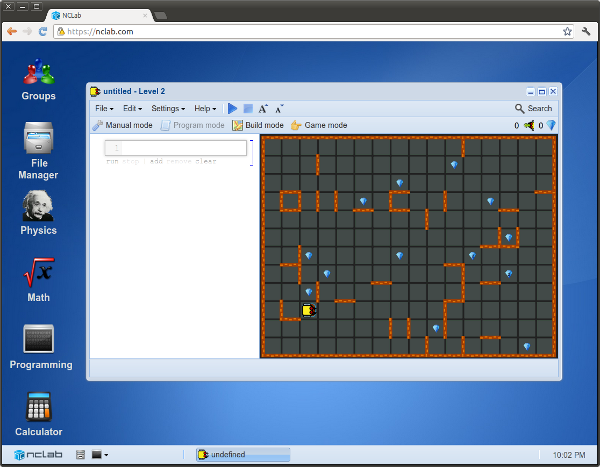
\includegraphics[width=\textwidth]{img/init.png}
\end{center}
\vspace{-2mm}
\caption{Launching Karel via the Programming icon.}
\label{fig:init}
%\vspace{-4mm}
\end{figure}
\noindent
Karel will be launched in {\em Programming mode} which is the most-frequently 
used one. You can easily switch to the {\em Manual mode}, {\em Build mode},
and {\em Game mode} in the menu. These modes will be discussed in Paragraph 
\ref{levels}.

\subsection{Karel's window} \label{menu}

The application window contains two lines of menus and information on top,
work area on the left, maze on the right, and status bar on the bottom.
The menus are fairly intuitive, so let us just explain a few selected functions, starting 
with the {\em File} menu:

{\em Open} will open a file from your NCLab account (not from your hard disk). {\em New} will generate a new random maze.
{\em Clone} will copy a Displayed Project into your account (to be discussed in Paragraph \ref{cloning}). 
{\em Display} will submit your project for review. If you think that 
      other users would find your program or game interesting, this is the way to make it 
      available to them. Upon passing the review, your project will be added to Displayed Projects.

{\em Edit} menu allows you to operate with input and text cells (to be discussed in 
Section \ref{sec:editmenu}). In {\em Settings} you can change Karel's {\em Level} (to be discussed
in Paragraph \ref{levels}), change his speed, and adjust sound preferences. The blue arrow and square 
buttons are used to run and stop programs, and the two buttons next to them can be used to increase and decrease 
font size. The pair of icons on far right is the step counter (that can be reset by clicking on it) and 
gem counter that indicates how many gems Karel has in his bag.

\subsection{Cloning Displayed Projects} \label{cloning}

All programs and exercises that we will work with are available for you to clone. 
To do this, click on {\em Clone} in Karel's File menu. This will launch a new window 
with Displayed Projects as shown in Fig. \ref{fig:cloning}.

\begin{figure}[!ht]
\begin{center}
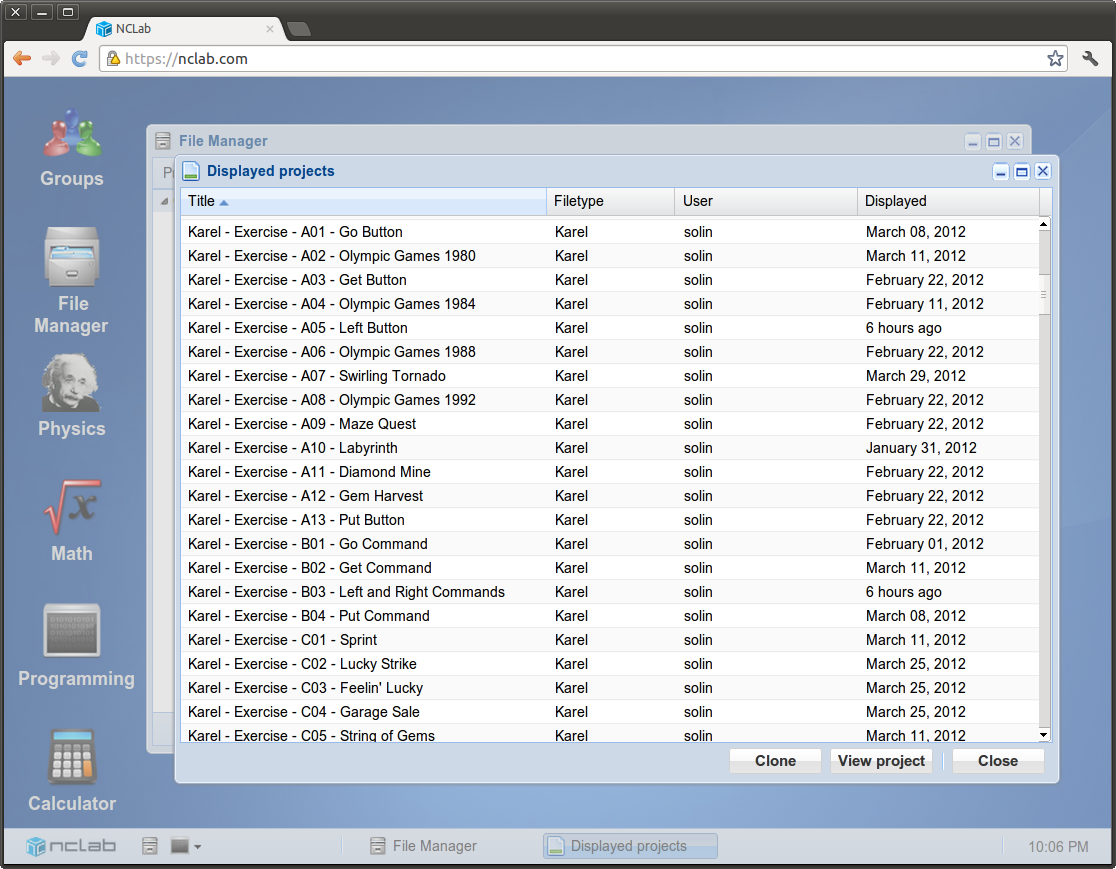
\includegraphics[width=\textwidth]{img/cloning.png}
\end{center}
%\vspace{-2mm}
\caption{Many exercises and games are available through the File menu.}
\label{fig:cloning}
\end{figure}
\newpage
\noindent
All projects whose names start with "Karel - Exercise" are of particular interest 
for this tutorial. Their solutions have names starting with "Karel - Solution". 
Any of them can be cloned into your account via clicking on the project name in the window, 
and pressing the button {\em Clone}.

In the File Manager's right-hand side panel, you will see the list of all 
projects that you cloned. Click on any of them to launch it. You are free to 
use the cloned projects as they are, or modify them in any way you like. Your 
modifications will not affect the original. And, you can 
always synchronize your version with the original, via 
a right-click on the project in the File Manager and selecting {\em Synchronize}.
Keep in mind though -- synchronizing with the original will erase any changes that 
you made to the project.

\subsection{Karel modes} \label{levels}

Karel operates in four modes:
\begin{itemize}
\item {\em Manual mode:} The robot is controlled using the mouse and five buttons Go, Get, Left, Right, and Put. 
      Watch out and do not crash!
\item {\em Program mode:} The robot is controlled using written programs (computer code). The Program mode is 
      split into several Levels:
\begin{itemize}
\item Level 1 is a transition layer between the Manual and Programming modes. Programs are written using only 
      five commands {\tt go}, {\tt get}, {\tt left}, {\tt right}, and {\tt put} that exactly correspond to 
      the buttons Go, Get, Left, Right, and Put in Manual mode.
\item Level 2 is where the actual programming begins. On top of the commands from Level 1, programs can contain 
      conditions, loops, and custom commands.
\item In Level 3 Karel furthermore receives a GPS device. The user will learn to work with logical 
      and numerical variables. 
\item Level 4 will teach the basics of object-oriented programming. This Level is in preparation.
\item Level 5 will teach the basics of parallel programming. This Level is in preparation.
\end{itemize}
\item {\em Build mode:} This mode allows the user to create custom mazes.
\item {\em Game mode:} Makes it possible to create and play games. 
\end{itemize}

\subsection{Review questions}

\begin{enumerate}
\item What can you do with a displayed Karel project that you clone into your account?.
\begin{enumerate}
\item[A1] View but not run.
\item[A2] View and run but not edit.
\item[A3] View, run and edit but not save.
\item[A4] View, run, edit, save, whatever, they are all yours!
\end{enumerate}
\item What are the four modes of the Karel application?
\begin{enumerate}
\item[A1] Manual mode, Build mode, Program mode, Game mode.
\item[A2] Mode 1, Mode 2, Mode 3, Mode 4.
\item[A3] Beginner mode, Intermediate mode, Advanced mode, Expert mode.
\item[A4] Karel has no modes.
\end{enumerate}
\item What is the difference between Levels 1 and 2?
\begin{enumerate}
\item[A1] In Level 2 the robot has more sensors. 
\item[A2] In Level 2 one can only guide the robot with the mouse.
\item[A3] In Level 2 one can only use 5 commands.
\item[A4] In Level 2 programs can contain 
      conditions, loops, and custom commands.
\end{enumerate}
\end{enumerate}


\section{Section A - Operating the Robot in Manual Mode}

\subsection{Objectives} 
\begin{itemize}
\item Learn to operate the robot in Manual mode.
\end{itemize}
\noindent
Before we begin, let us review the four directions on the compass:

\begin{figure}[!ht]
\begin{center}
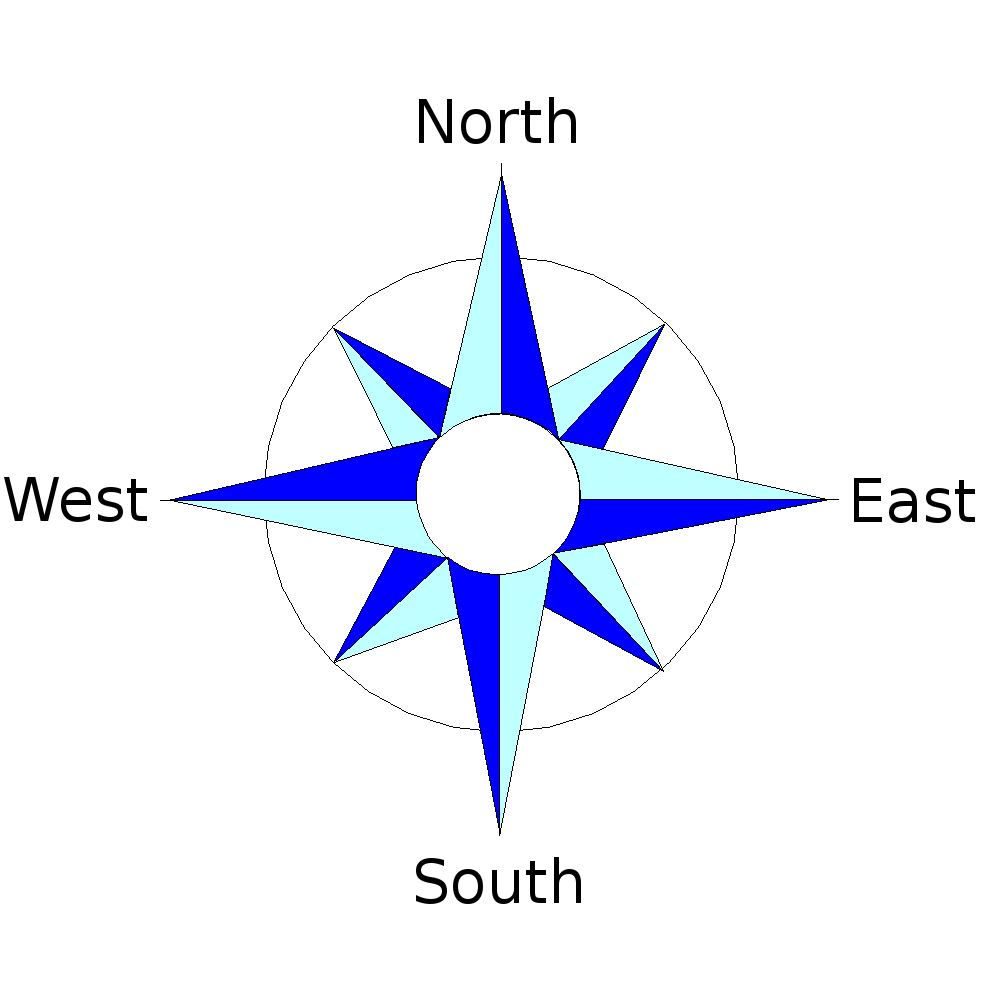
\includegraphics[width=0.5\textwidth]{img/compass.png}
\vspace{-0mm}
%\caption{Karel's four possible orientations.}
%\label{fig:ori}
\end{center}
\vspace{-1cm}
\end{figure}
\noindent
When launching Karel through the Programming icon, switch to Manual mode using the corresponding 
menu button. Then, five buttons Left, Right, Go, Get and Put will appear in the panel on the left,
as shown in Fig. \ref{fig:buttons}.

\newpage

\begin{figure}[!ht]
\begin{center}
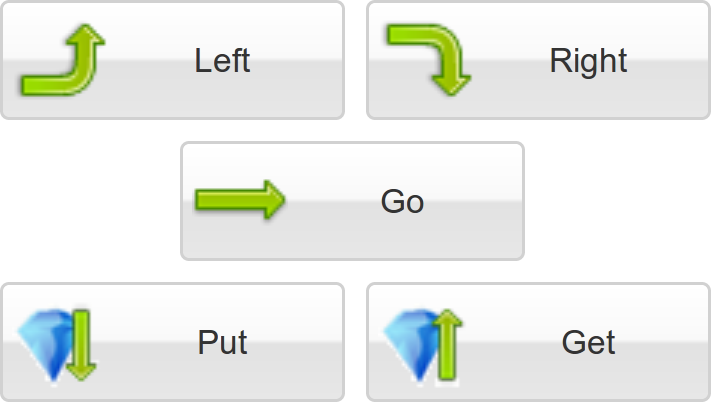
\includegraphics[width=6.2cm]{img/buttons-all.png}
\vspace{-0mm}
\caption{Karel's buttons in manual mode (robot facing East).}
\label{fig:buttons}
\end{center}
\end{figure}
\noindent
The function of the buttons is self-explanatory -- pressing Left will turn the robot 90 degrees to the left,
pressing Right will turn him 90 degrees to the right, and pressing Go will move him one step forward 
(watch out and do not crash into a wall!). Upon pressing Put the robot will reach into his bag with gems, 
take one, and put it on the ground where he stands. Make sure that the bag is not empty before you do this!
An indicator showing how many gems are in the bag is in the upper right corner of the window. Last, upon pressing 
Get the robot will pick up a gem from the ground where he stands. Before you ask the robot to get a gem,
make sure that there is a gem on the ground though, or he will get annoyed!

When the robot turns, the arrows on the buttons adjust automatically to his new 
orientation. This is illustrated in Fig. \ref{fig:buttons2}.
\begin{figure}[!ht]
\begin{center}
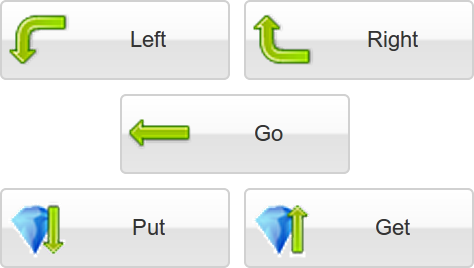
\includegraphics[width=6.2cm]{img/buttons-all-2.png}
\vspace{-0mm}
\caption{Karel's buttons in manual mode (robot facing West).}
\label{fig:buttons2}
\end{center}
\end{figure}

\noindent
When you first clone a Karel Exercise ("A" section contains 
games in manual mode) and then 
run it, there is not even need to switch to Manual mode -- just press the Start button and you are 
all set.

\subsection{Review questions}

\begin{enumerate}
\item How can Karel be switched to Manual mode?
\begin{enumerate}
\item[A1] Through Settings in main manu.
\item[A2] By pressing the Program mode twice
\item[A3] By pressing the Manual mode button.
\item[A4] Through the File menu.
\end{enumerate}
\item Look at  the arrows and decide which direction the robot is facing!
\begin{figure}[!ht]
\begin{center}
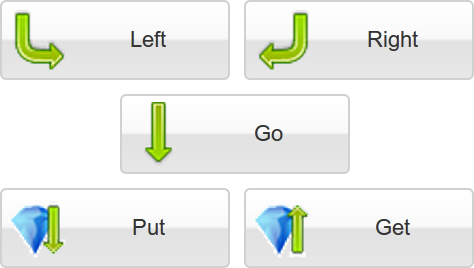
\includegraphics[width=6.2cm]{img/buttons-all-3.png}
\end{center}
\end{figure}
\begin{enumerate}
\item[A1] North.
\item[A2] South.
\item[A3] East.
\item[A4] West.
\end{enumerate}
\item What is the function of the following button?

\begin{figure}[!ht]
\begin{center}

\includegraphics[width=3cm]{img/button-left-1.png}
\end{center}
\end{figure}
\begin{enumerate}
\item[A1] Make one step forward, turn left, and make one step forward.
\item[A2] Make one step forward and turn left
\item[A3] Step aside towards East and then make one step forward.
\item[A4] Turn left.
\end{enumerate}
\item Select one or more correct statements from the four options below!
\begin{figure}[!ht]
\begin{center}

\includegraphics[width=3cm]{img/button-left-1.png}\ \ \

\includegraphics[width=3cm]{img/button-left-2.png}\ \ \

\includegraphics[width=3cm]{img/button-left-3.png}\ \ \

\includegraphics[width=3cm]{img/button-left-4.png}
\end{center}
\end{figure}

\begin{enumerate}
\item[A1] All these buttons will turn the robot 90 degrees to the right.
\item[A2] Two of the buttons will turn the robot to the left, the other two will turn him to the right.
\item[A3] The last button on the right will turn the robot to the left.
\item[A4] The last button on the right will turn the robot to the right.
\end{enumerate}
\item After you press the following button, the robot will:

\begin{figure}[!ht]
\begin{center}

\includegraphics[width=3cm]{img/button-right-4.png}
\end{center}
\end{figure}
\begin{enumerate}
\item[A1] Turn left and face West.
\item[A2] Turn right and face West.
\item[A3] Turn right and face East
\item[A4] Turn right and face South.
\end{enumerate}
\end{enumerate}
There are thirteen exercises A01 - A13 for you to solve.
Each exercise can be cloned via the File Manager's 
{\em Project} menu as described in Paragraph \ref{cloning}. 
Do not skip levels since they are very simple and each one has something new! 

\newpage
\subsection{Exercise A01 - Go Button}

{\em Karel is returning from a long walk and his batteries are running out. 
Use the buttons on the left to get him home quickly! }

\begin{figure}[!ht]
\begin{center}
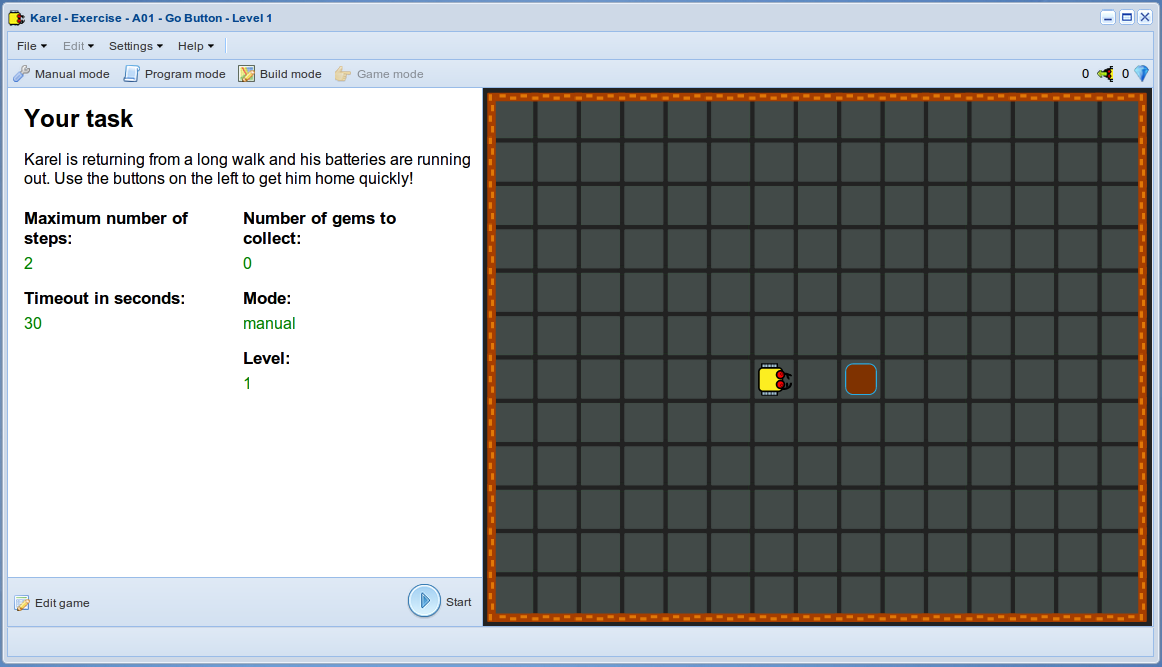
\includegraphics[height=0.4\textwidth]{img/a01.png}
\end{center}
\vspace{-4mm}
\caption{In the first exercise you need to help the robot get home.}
\label{fig:a01}
\end{figure}
\noindent
Pressing Start will start 
the exercise, and at this time also the buttons Go, Left, Right, Put and Get appear, 
as shown in Fig. \ref{fig:a01b}.


\begin{figure}[!ht]
\begin{center}
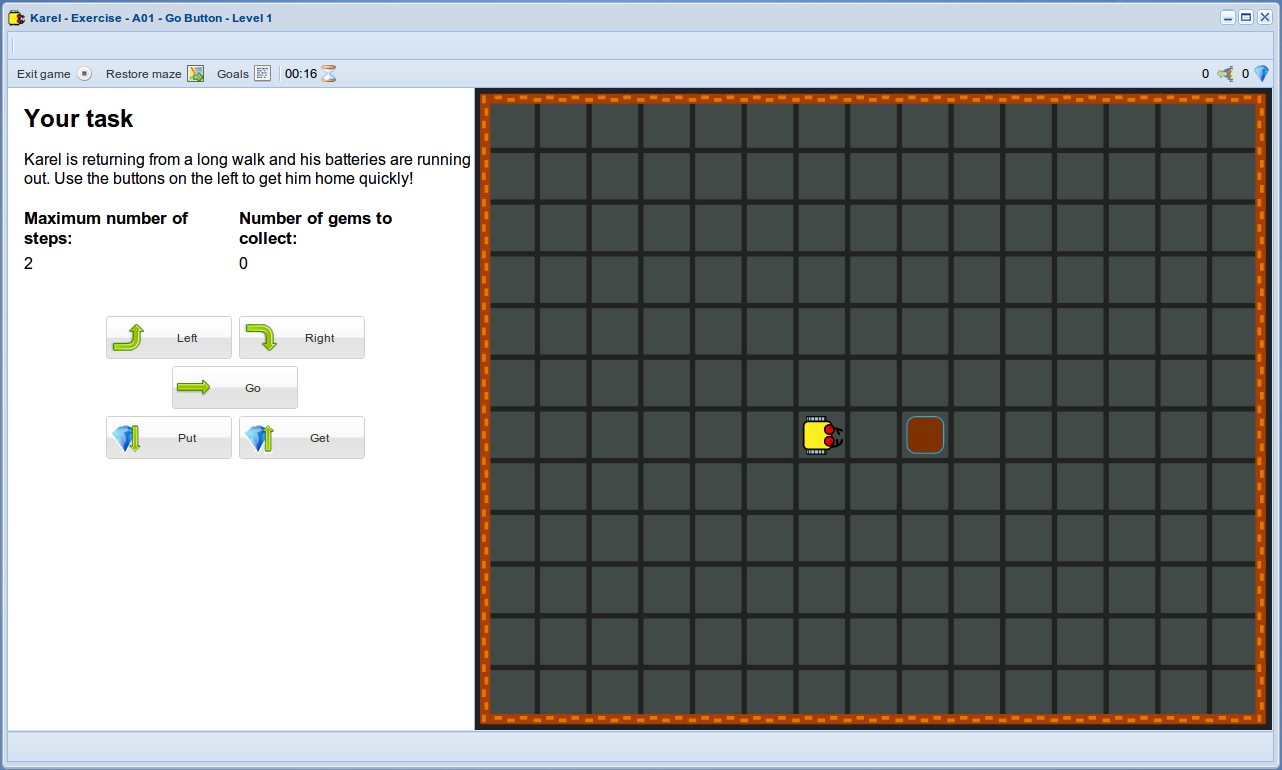
\includegraphics[height=0.4\textwidth]{img/a01b.png}
\end{center}
\vspace{-4mm}
\caption{Karel can be guided manually, using five buttons located in the left panel.}
\label{fig:a01b}
\end{figure}


\subsection{Exercise A02 - Olympic Games 1980}

{\em Karel is training for Robolympic Games! Your task is to run with 
the robot home as fast as possible. Karel's personal record is four seconds. How fast can you be?}

\begin{figure}[!ht]
\begin{center}
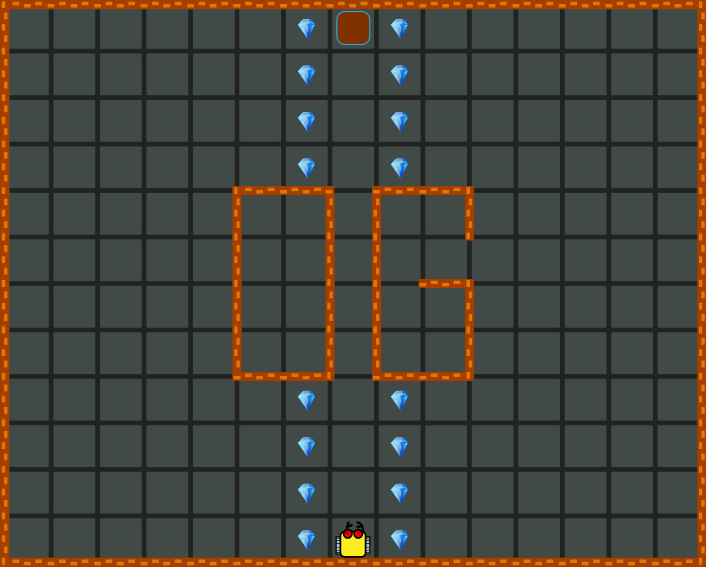
\includegraphics[height=0.4\textwidth]{img/a02.png}
\end{center}
\vspace{-4mm}
\caption{Karel is training for Robolympic Games.}
\label{fig:a02}
\vspace{-4mm}
\end{figure}
\noindent

\subsection{Exercise A03 - Get Button}

{\em Today is Karel's lucky day because he is about to find his first gem. 
Use the buttons on the left to help the robot pick up the gem and carry it 
home!}

\begin{figure}[!ht]
\begin{center}
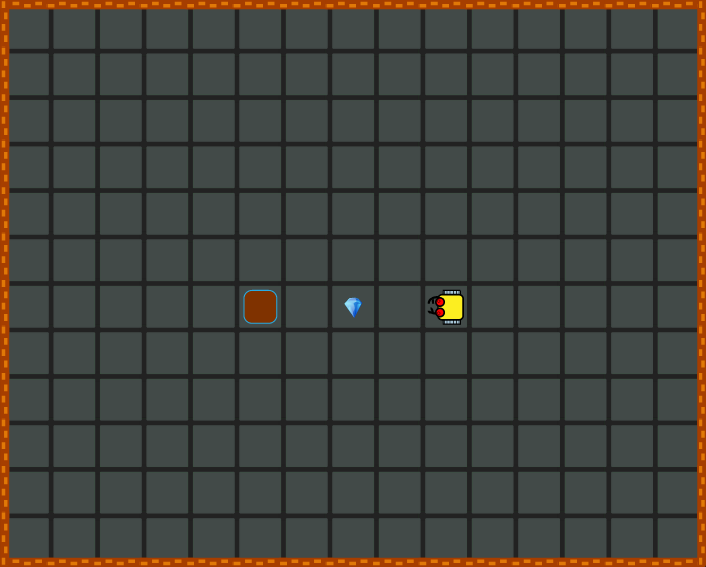
\includegraphics[height=0.4\textwidth]{img/a03.png}
\end{center}
\vspace{-4mm}
\caption{Karel is about to find his first gem.}
\label{fig:a03}
\vspace{-1cm}
\end{figure}
\noindent

\newpage
\subsection{Exercise A04 - Olympic Games 1984}

{\em It is Robolympic season again! Run home as fast as you can, 
and collect all three gems on the way! Karel's personal record is 10 seconds.}


\begin{figure}[!ht]
\begin{center}
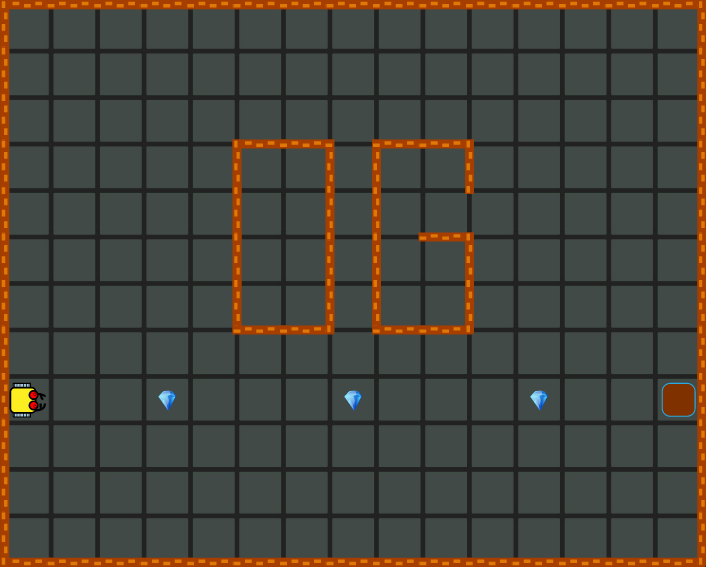
\includegraphics[height=0.4\textwidth]{img/a04.png}
\end{center}
\vspace{-4mm}
\caption{Karel's second Robolympic Games.}
\label{fig:a04}
\vspace{-1cm}
\end{figure}
\noindent


\subsection{Exercise A05 - Left Button}

{\em Help the robot collect the gem and return home!}

\begin{figure}[!ht]
\begin{center}
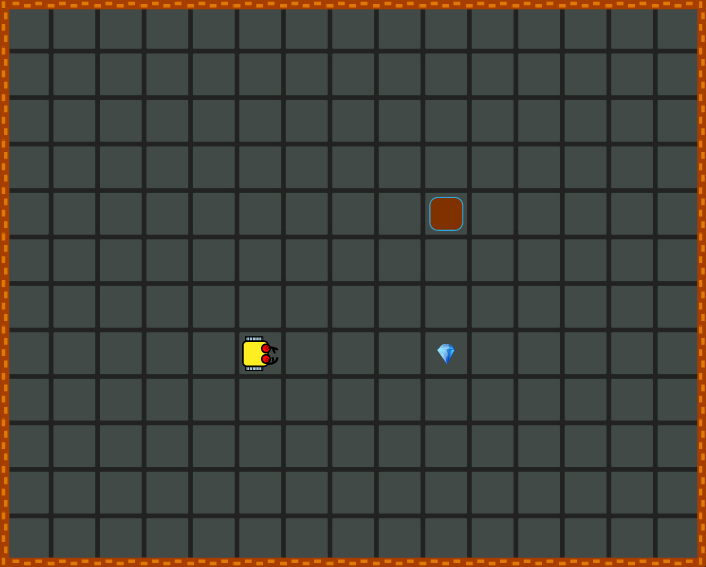
\includegraphics[height=0.4\textwidth]{img/a05.png}
\end{center}
\vspace{-4mm}
\caption{Karel is about to learn how to make a left turn.}
\label{fig:a05}
\vspace{-1cm}
\end{figure}
\noindent

\newpage

\subsection{Exercise A06 - Olympic Games 1988 }

{\em Karel is training for his third Robolympic Games. Run with him around the block and home as fast as possible. He needs to collect at least one gem on the way. Karel's personal record is 16 seconds!}

\begin{figure}[!ht]
\begin{center}
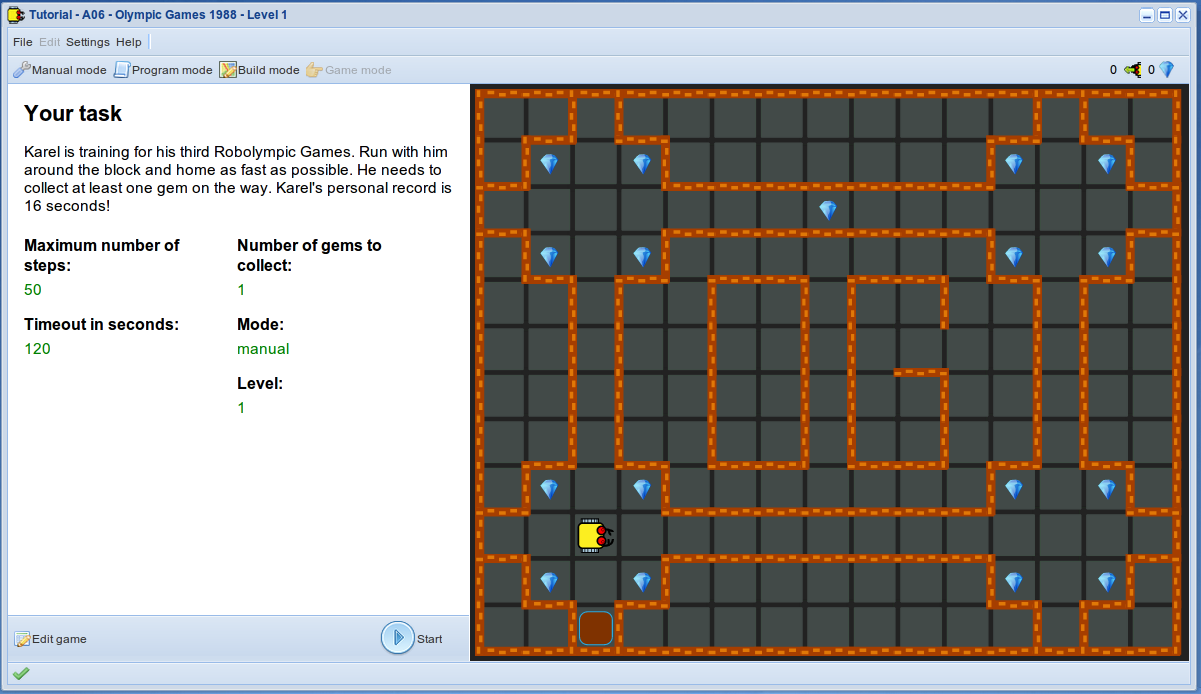
\includegraphics[height=0.4\textwidth]{img/a06.png}
\end{center}
\vspace{-4mm}
\caption{Karel's third Robolympic Games.}
\label{fig:a06}
\vspace{-1cm}
\end{figure}
\noindent


\subsection{Exercise A07 - Right Button}

{\em Pick up the two gems and get Karel home!}

\begin{figure}[!ht]
\begin{center}
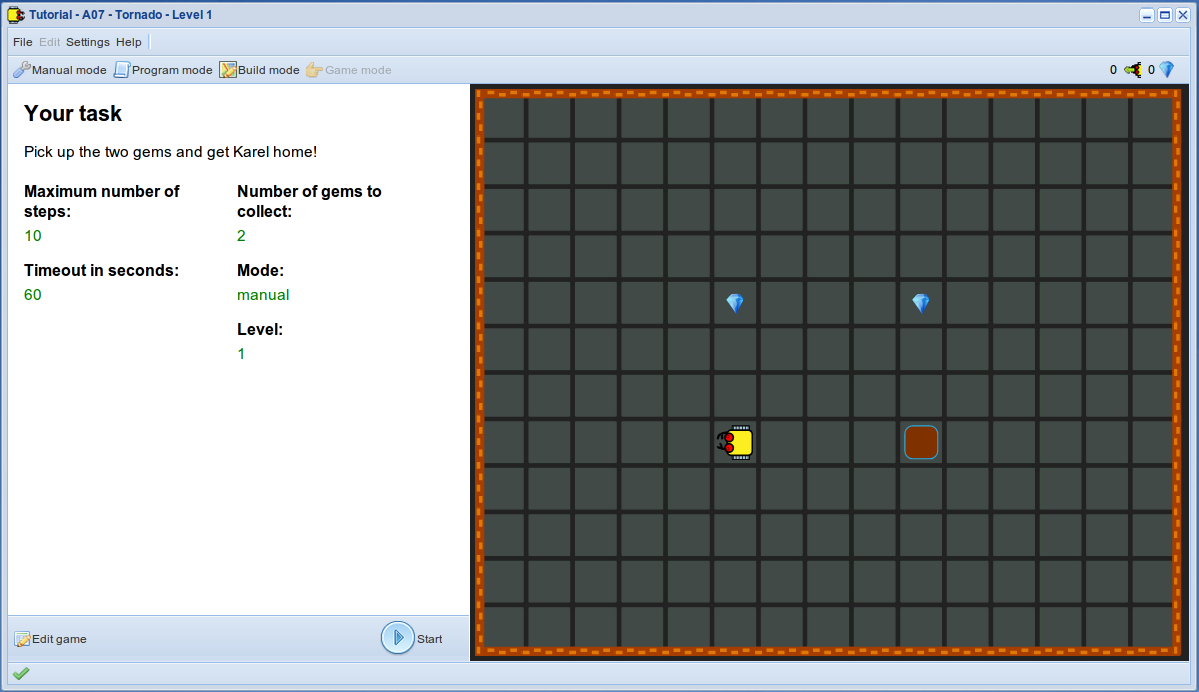
\includegraphics[height=0.4\textwidth]{img/a07.png}
\end{center}
\vspace{-4mm}
\caption{Karel needs to collect two gems and get home.}
\label{fig:a07}
\vspace{-1cm}
\end{figure}
\noindent
\newpage

\subsection{Exercise A08 - Olympic Games 1992}

{\em Last season of Karel's Robolympics Games is here! The 
robot needs to run home as fast as possible and bring one gem. 
Be careful not to crash, this is a tricky level! Karel's personal record is 26 seconds.}\\[-7mm]

\begin{figure}[!ht]
\begin{center}
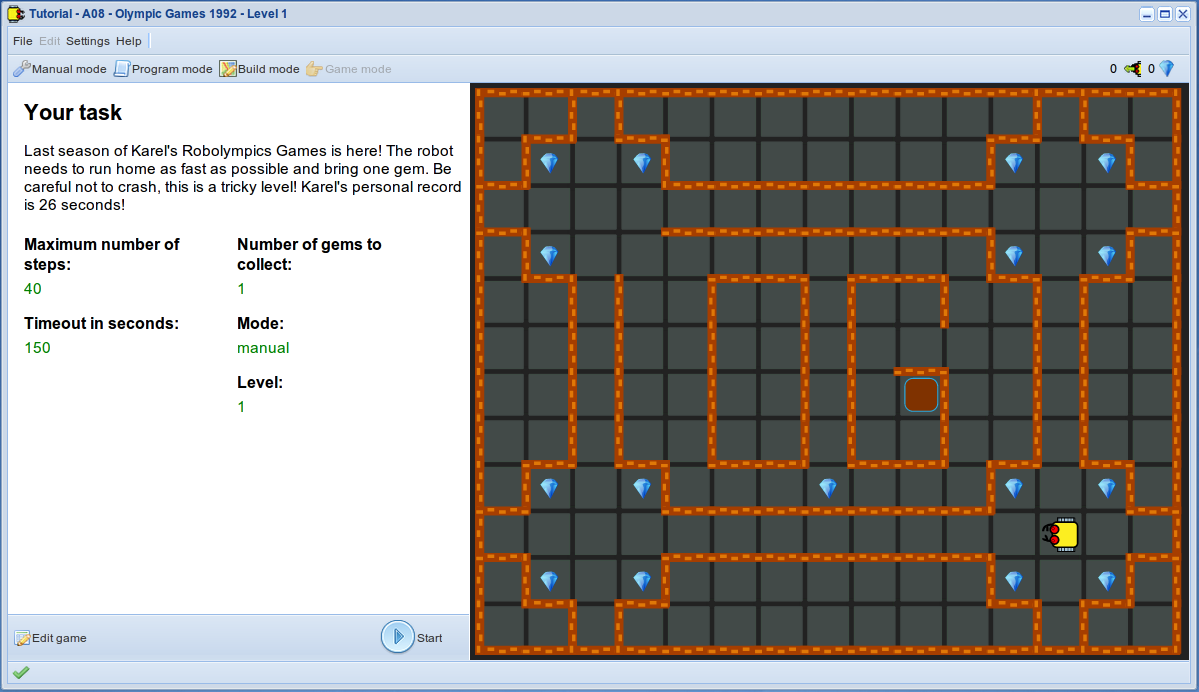
\includegraphics[height=0.4\textwidth]{img/a08.png}
\end{center}
\vspace{-4mm}
\caption{Karel's fourth Robolympic Games.}
\label{fig:a08}
\vspace{-4mm}
\end{figure}
\noindent

\subsection{Exercise A09 - Maze Quest}

{\em This time Karel got seriously lost while looking for his favorite gem. 
Help him to collect the gem and find his way home!}\\[-7mm]

\begin{figure}[!ht]
\begin{center}
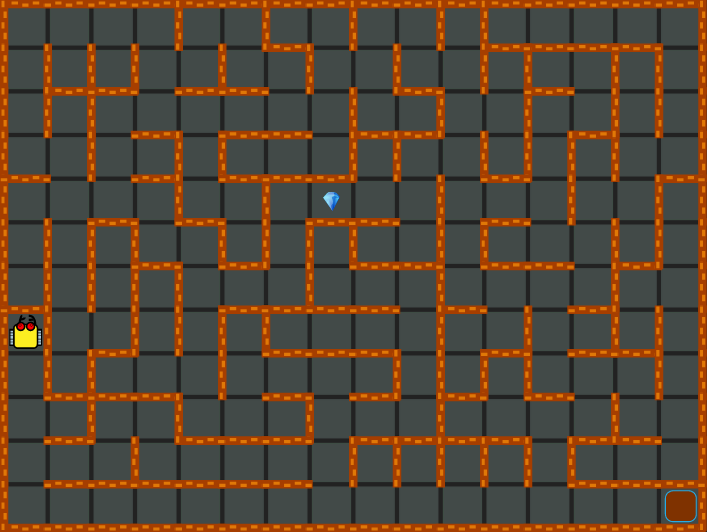
\includegraphics[height=0.4\textwidth]{img/a09.png}
\end{center}
\vspace{-4mm}
\caption{Karel got lost while looking for his favorite gem.}
\label{fig:a09}
\vspace{-4mm}
\end{figure}
\noindent
\newpage

\subsection{Exercise A10 - Labyrinth}

{\em This is a true labyrinth and your task is to lead Karel 
home. Remember - think first before going anywhere!}

\begin{figure}[!ht]
\begin{center}
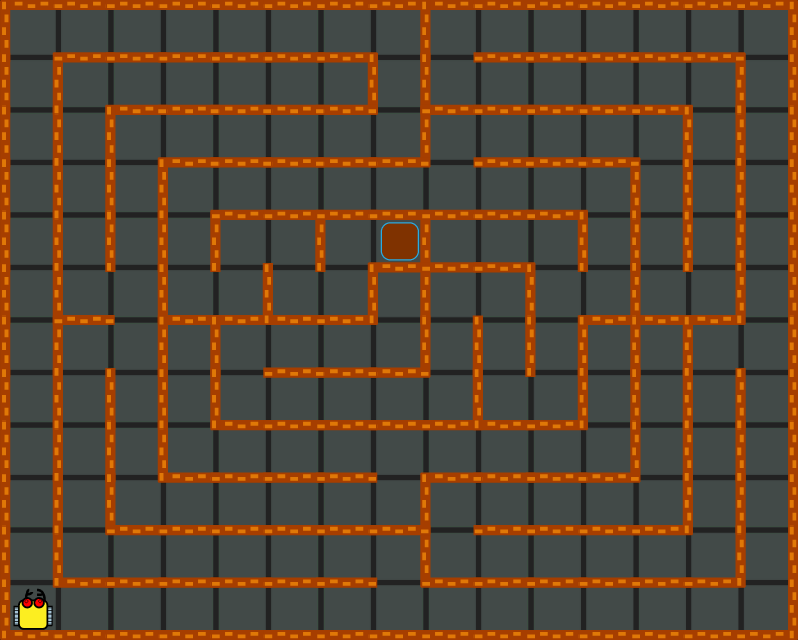
\includegraphics[height=0.4\textwidth]{img/a10.png}
\end{center}
\vspace{-4mm}
\caption{Karel needs to find his way home in a labyrinth.}
\label{fig:a10}
\vspace{-4mm}
\end{figure}
\noindent


\subsection{Exercise A11 - Diamond Mine}

{\em Karel discovered an abandoned diamond mine. Use the buttons
on the left to collect all gems and get back home in time!}

\begin{figure}[!ht]
\begin{center}
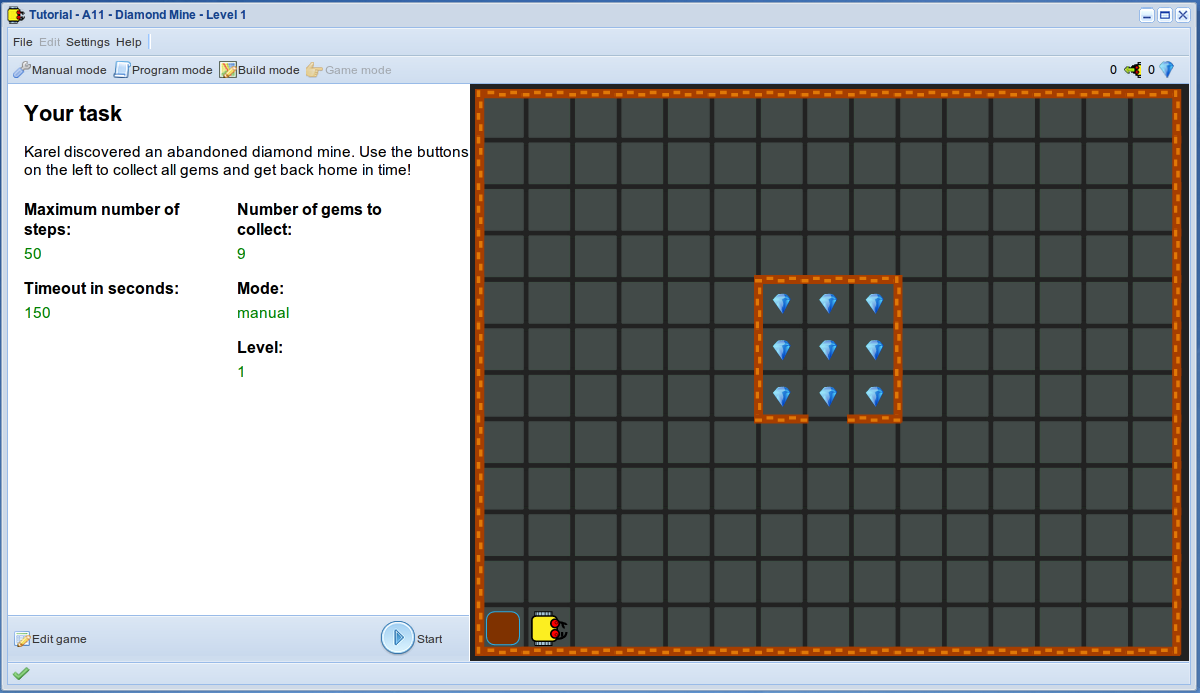
\includegraphics[height=0.4\textwidth]{img/a11.png}
\end{center}
\vspace{-4mm}
\caption{Karel found an abandoned diamond mine.}
\label{fig:a11}
\vspace{-4mm}
\end{figure}
\noindent
\newpage

\subsection{Exercise A12 - Gem Harvest}

{\em If gems are piled up, then a number is showing their amount. 
Help Karel collect all gems in this maze and return home!}\\[-7mm]

\begin{figure}[!ht]
\begin{center}
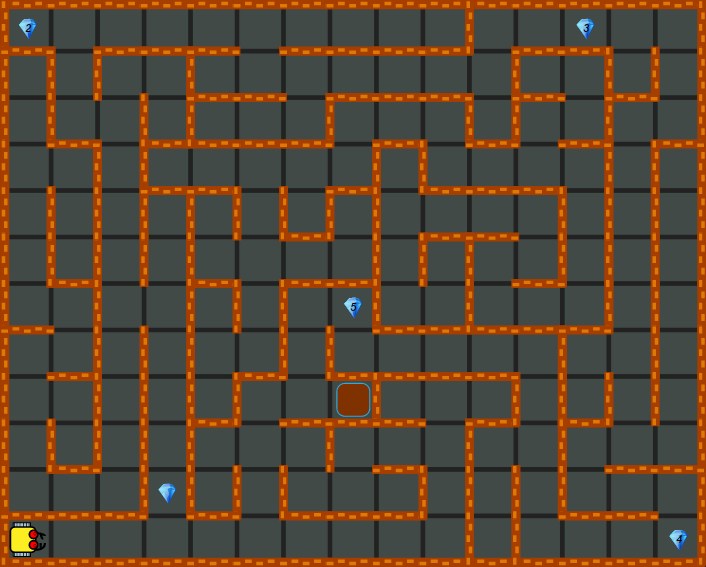
\includegraphics[height=0.4\textwidth]{img/a12.png}
\end{center}
\vspace{-4mm}
\caption{If gems are piled up, then a number is showing their amount.}
\label{fig:a12}
\vspace{-4mm}
\end{figure}
\noindent


\subsection{Exercise A13 - Put Button}

{\em Karel has five gems in his bag. Use the buttons on the left to put the gems on the table and 
return home in time!}\\[-7mm]

\begin{figure}[!ht]
\begin{center}
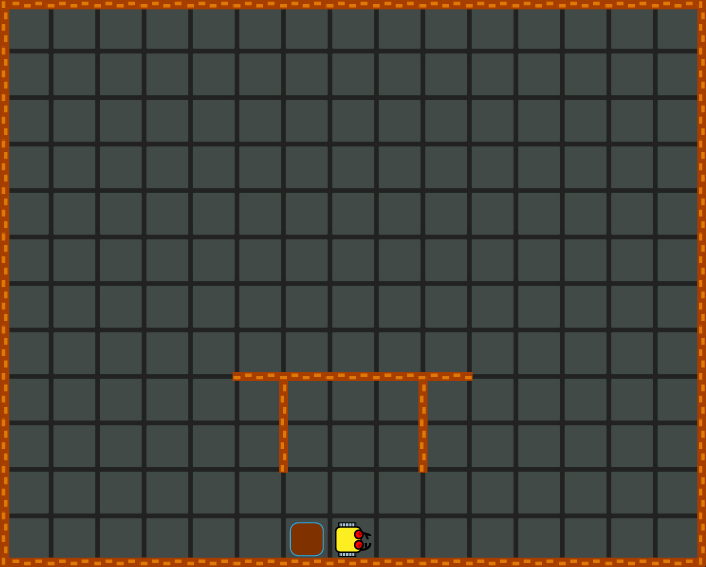
\includegraphics[height=0.4\textwidth]{img/a13.png}
\end{center}
\vspace{-4mm}
\caption{Karel needs to put five gems on the table.}
\label{fig:a13}
\vspace{-4mm}
\end{figure}
\noindent
\newpage

\section{Section B - Bridge to Programming}

\subsection{Objectives} 
 
\begin{itemize}
\item Start operating the robot in Programming mode.
\end{itemize}
In Programming mode, commands for the robot are entered into an input cell located in the left panel.
These commands are {\tt left}, {\tt right}, {\tt go}, {\tt get}, and {\tt put}.
Their function is the same as the function of the corresponding buttons in Manual mode.
One or more commands form a {\em computer program (computer code)}. Often 
we just say {\em program} or {\em code}.

There are two simple rules to remember:
\begin{enumerate}
\item Always type one command per line.
\item Do not enter empty characters in front of commands. 
\end{enumerate}
Ignoring these rules would not make your program invalid, but your code would be 
difficult to read. It is important to write a clean, transparent code that is easy to read. 

\subsection{Review questions}

\begin{enumerate}
\item Where do we enter programs for Karel?
\begin{enumerate}
\item[A1] In Microsoft Word.
\item[A2] In DreamWeaver.
\item[A3] We upload them from hard disk.
\item[A4] In input cells.
\end{enumerate}
\item Do we have to write one command per line?
\begin{enumerate}
\item[A1] Yes, otherwise the program would not run.
\item[A2] No, but any commands beyond the first are ignored.
\item[A3] No, but it makes the code easier to read.
\item[A4] Yes, otherwise the program would not work correctly.
\end{enumerate}
\item The robot's initial situation is as shown in the image. His bag with gems is empty.
\begin{figure}[!ht]
\begin{center}
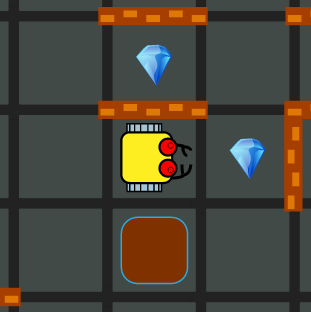
\includegraphics[width=4cm]{img/maze-0.png}
\end{center}
\end{figure}
\newpage
\noindent
Read the following program and select one or more correct statements!
\begin{verbatim}
go
right
get
go
right 
go
\end{verbatim}
\begin{enumerate}
\item[A1] The robot will return home with no gems in thebag.
\item[A2] The robot will return home with one gem in thebag.
\item[A3] The robot will not return home and he will have no gems in the bag.
\item[A4] The robot will not return home and he will have one gem in the bag.
\end{enumerate}
\item The robot's initial situation is the same as in the previous question. He has not gems 
in his bag. Read the following program and select one or more correct statements from the four options below!
\begin{verbatim}
go
get
left
go
left
go
get
right
right
go
right
go
put
go
left 
go
\end{verbatim}
\begin{enumerate}
\item[A1] The robot will return home with two gems in the bag.
\item[A2] The robot will return home with only one gem in the bag.
\item[A3] The robot will not return home and he will have two gems in the bag.
\item[A4] The robot will not return home and he will have only one gem in the bag.
\end{enumerate}
\end{enumerate}
Before continuing, please clone into your account all exercises from the B-Section via the File Manager's {\em Project}
menu.

\newpage
\subsection{Exercise B01 - Go Command}

{\em Write a program that gets Karel home! Remember: Always write one command per line.}

\begin{figure}[!ht]
\begin{center}
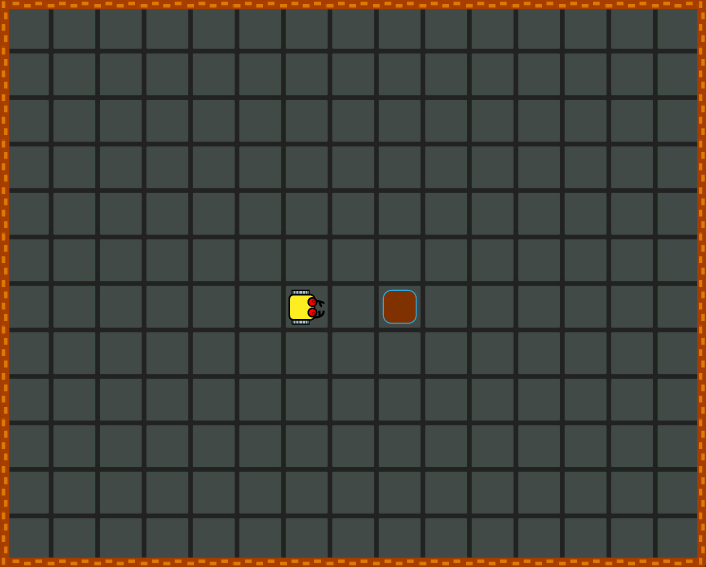
\includegraphics[height=0.4\textwidth]{img/b01.png}
\end{center}
\vspace{-4mm}
\caption{Moving Karel forward via the {\tt go} command.}
\label{fig:b01}
\vspace{-4mm}
\end{figure}
\noindent

\subsection{Exercise B02 - Get Command}

{\em Write a program for Karel to collect all gems and get home! 

\begin{figure}[!ht]
\begin{center}
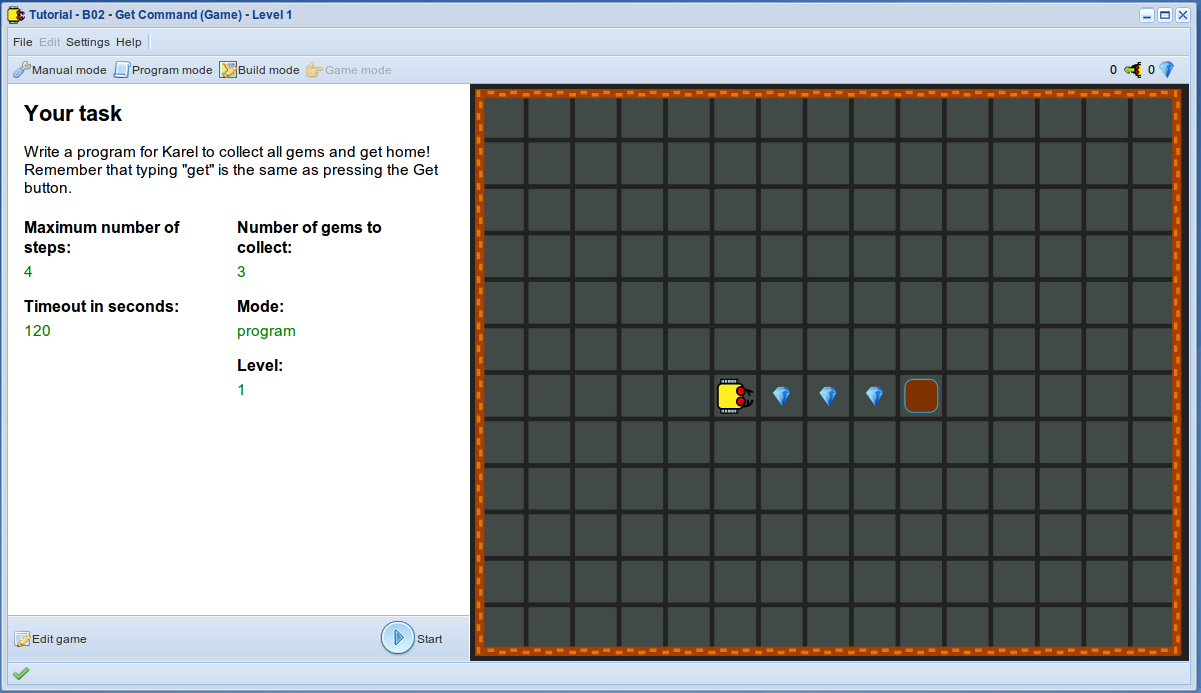
\includegraphics[height=0.4\textwidth]{img/b02.png}
\end{center}
\vspace{-4mm}
\caption{Collecting gems using the {\tt get} command.}
\label{fig:b02}
\vspace{-4mm}
\end{figure}
\noindent

\newpage

\subsection{Exercise B03 - Left and Right Commands}

{\em Write a program for Karel to collect the gem and return home! 

\begin{figure}[!ht]
\begin{center}
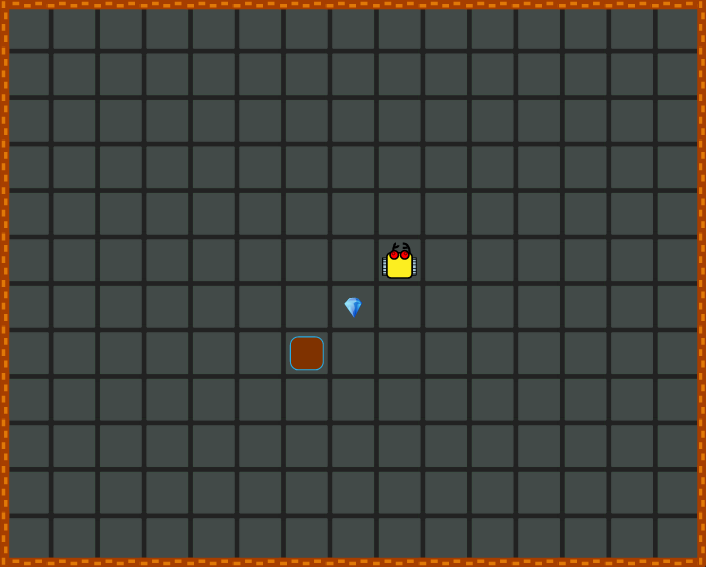
\includegraphics[height=0.4\textwidth]{img/b03.png}
\end{center}
\vspace{-4mm}
\caption{Turning to the left and to the right via the {\tt left} and {\tt right} commands.}
\label{fig:b03}
\vspace{-4mm}
\end{figure}
\noindent

\subsection{Exercise B04 - Put Command}

{\em Write a program for Karel to relocate the gem to the opposite 
end of the cross and return home!}



\begin{figure}[!ht]
\begin{center}
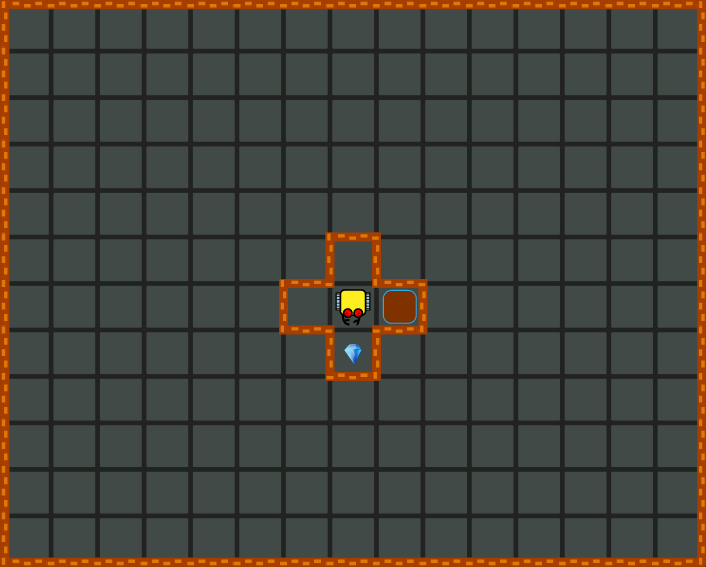
\includegraphics[height=0.4\textwidth]{img/b04.png}
\end{center}
\vspace{-4mm}
\caption{Relocating a gem requires both {\tt get} and {\tt put} commands.}
\label{fig:b04}
\vspace{-4mm}
\end{figure}
\noindent
\newpage

\section{Intermission - Algorithms, Programs, and Bugs}

\subsection{Objectives} 
 
\begin{itemize}
\item Understand the difference between {\em algorithm} and {\em program}. 
\item Learn the difference between {\em syntactical} and {\em logical} mistakes.
\item Understand that {\em debugging} is an indivisible part of computer programming.
\end{itemize}
Karel always obeys all commands {\em precisely}. Sometimes it may happen that 
we plan one thing but to our surprise the robot does something else. In most cases this 
happens when our {\em algorithm} is wrong. By an {\em algorithm} we mean a sequence of 
logical steps that the robot needs to follow in order to fulfill his task. Algorithms 
are presented using normal human language, not in terms of the robot's commands. 

{\em Program} or {\em computer code} is created when the algorithm is expressed
in terms of the robot's language. When our algorithm is good, then 
the program is easy to write.

Mistakes in algorithms are called {\em logical errors}. A logical error is, for 
example, when we crash the robot into a wall because we forgot to make a turn.
Mistakes such as mis-spelling a command, writing "1o" instead of "10", or forgetting 
indentation are related to 
{\em syntax} and they are called {\em syntactical errors}. Of these two types, 
logical errors are usually much more difficult to find. 

In general, mistakes or either kind are called {\em bugs} and the procedure of 
eliminating them is called {\em debugging}. Depending on how careful we 
were while preparing our algorithm and writing the program, debugging takes either 
a short time or a long time. It does not happen often that a program works correctly
right away. 

When we commit a syntactical error,
the robot will write an error message and do nothing.
If our algorithm contains a logical error, then he will
write an error message and stop executing the program. 
The most usual logical error are:

\begin{itemize}
\item Karel crashes into a wall.
\item The robot tries to collect a gem where is none.
\item He attempts to put a gem on the ground while his bag is empty.
\end{itemize}

\subsection{Review questions} 

\begin{enumerate}
\item What is an {\em algorithm}?
\begin{enumerate}
\item[A1] Very short program.
\item[A2] Sequence of instructions for the robot written using the correct commands.
\item[A3] Logical mistake in our program.
\item[A4] Sequence of logical steps leading to the solution of the given task.
\end{enumerate}
\item What is a {\em program}?
\begin{enumerate}
\item[A1] Sequence of logical steps written using human language.
\item[A2] Algorithm that does not contain any mistakes.
\item[A3] Algorithm that is translated from human language to the robot's language.
\item[A4] Very long algorithm.
\end{enumerate}
\item If the robot does something unexpected, what is the most probable reason for that?
\begin{enumerate}
\item[A1] Something is wrong with the computer.
\item[A2] Internet connection is too slow.
\item[A3] Web browser needs upgrading.
\item[A4] Our algorithm contains a logical mistake.
\end{enumerate}
\item What of the following is a {\em logical} mistake?
\begin{enumerate}
\item[A1] Mistake in an algorithm that causes the robot to do something unexpected.
\item[A2] Opening Karel through the Programming menu instead of through File Manager. 
\item[A3] Typing a command in a wrong way, such as {\tt lft} instead of {\tt left}.
\item[A4] Learning Fortran.
\end{enumerate}
\item What of the following is a {\em syntactical} mistake?
\begin{enumerate}
\item[A1] Writing two commands on the same line.
\item[A2] Having two empty characters between commands.
\item[A3] Mis-spelling a command.  
\item[A4] Mistake that causes the robot to do something unexpected.
\end{enumerate}
\item What of the following will cause an error message?
\begin{enumerate}
\item[A1] Turning the robot four times to the left or right.
\item[A2] Putting two or more gems on each other.
\item[A3] Putting a gem while the bag is empty.
\item[A4] Returning home without any gems.
\end{enumerate}
\item What do we mean by {\em debuging}?
\begin{enumerate}
\item[A1] Apologizing after we ask a friend too many questions.
\item[A2] Playing an algorithm in our head prior to writing a program. 
\item[A3] Looking for mistakes when our program does not work.
\item[A4] Writing a new program after the previous one did not work.
\end{enumerate}
\end{enumerate}

\section{Section C - Counting Loop}

\subsection{Objectives} 

\begin{itemize}
\item Learn to make the robot repeat something a given number of times.
\end{itemize}

\noindent
In Section B we successfully crossed the bridge between manual control 
and programming. The bridge collapsed, there is no way back. But do 
not worry about that! The land of Programming is much more beautiful,
and once you understand its beauty, you will never want to leave.


\subsection{The {\tt repeat} command}

The {\em counting loop}, represented by the {\tt repeat} command, can save 
us lots of writing when something is repeated a given number of times. 
For example, for Karel to make 15 steps forward we could type:

\begin{verbatim}
go
go
go
go
go
go
go
go
go
go
go
go
go
go
go
\end{verbatim}
But this is neither efficient nor elegant. Instead, the same can be
achieved by telling Karel to {\tt repeat} the {\tt go} command {\tt 7} times:

\begin{verbatim}
repeat 15
  go
\end{verbatim}
There are a few simple rules that we need to remember when using the {\tt repeat} command:

\begin{itemize}
\item Keep code readable -- always write one command per line.
\item Indentation -- all commands to be repeated (the {\em body of the loop}) need to be indented. You can
      choose whether you prefer 2-indents or 4-indents. The former yields more compact 
      code with not-so-long lines, the latter is easier to read. 
\item Cancel the indentation for the first command that does not belong to the body of the loop.
\end{itemize}
To illustrate what the indentation does, let's look at a code that will move the robot 8 steps forward:

\begin{verbatim}
repeat 4
  go
  go
\end{verbatim}
Compare to a code that will only move the robot 5 steps forward:

\begin{verbatim}
repeat 4
  go
go
\end{verbatim}
Multiple {\tt repeat} commands can be {\em nested}. This means that a {\tt repeat} command 
can used in the body of another {\tt repeat} command. Everything that was said about indentation 
still holds. Can you figure out what the following code does?

\begin{verbatim}
repeat 10
  repeat 5
    go
  repeat 2
    left
\end{verbatim}
After you figure it out, launch Karel via the {\em Programming} menu, enter this code into
the input cell, and run it! But before you do, remember to switch to {\em Build mode} and make 
some free space in front of the robot 
so that he does not crash into a wall.

\subsection{Review questions} 

\begin{enumerate}
\item What command should we use to make the robot repeat something a given number of times?
\begin{enumerate}
\item[A1] {\tt repetition}
\item[A2] {\tt loop}
\item[A3] {\tt for}
\item[A4] {\tt repeat}
\end{enumerate}
\item Why should we always write one command per line?
\begin{enumerate}
\item[A1] To keep the code readable.
\item[A2] To make the code look longer.
\item[A3] Because all programming languages require that.
\item[A4] Because it speeds up communication with server.
\end{enumerate}
\item What is the {\em body of a loop}?
\begin{enumerate}
\item[A1] Body of a loop is the number that follows the {\tt repeat} command. 
\item[A2] The command on the first line following the {\tt repeat} command.
\item[A3] One or more commands that follow the {\tt repeat} command and are indented.
\item[A4] One or more commands that follow the {\tt repeat} command and are not indented.
\end{enumerate}
\item Why does the body of a loop need to be indented?
\begin{enumerate}
\item[A1] To make clear where the body of the loop begins and where it ends.
\item[A2] It does not have to be indented, the indentation is optional.
\item[A3] Because the code is visually nicer.
\item[A4] Because the code is easier to read.
\end{enumerate}
\item Which of the following programs will rotate Karel 360 degrees?
\begin{enumerate}
\item[A1] 
\begin{verbatim}
 left
 left
 left
 left
\end{verbatim}
\item[A2] 
\begin{verbatim}
 repeat 2
   right
   right
\end{verbatim}
\item[A3] 
\begin{verbatim}
 repeat 4
   left
\end{verbatim}
\item[A4] 
\begin{verbatim}
 repeat 2
   repeat 2
     right
\end{verbatim}
\end{enumerate}
\item Karel needs to pick up 5 gems from the ground, walk 10 steps forward, and put the 5 gems 
      on the ground again. Which ones of the following programs will do that?
\begin{enumerate}
\item[A1] 
\begin{verbatim}
 repeat 5
   get
   repeat 10
     go
     repeat 5
       put
\end{verbatim}
\item[A2] 
\begin{verbatim}
 repeat 5
   get
 repeat 10
   go
 repeat 5
   put
\end{verbatim}
\item[A3] 
\begin{verbatim}
 repeat 5
   get
   repeat 10
     go
   repeat 5
     put
\end{verbatim}
\item[A4] 
\begin{verbatim}
 repeat 5
 get
 repeat 10
 go
 repeat 5
 put
\end{verbatim}
\end{enumerate}
\end{enumerate}

\subsection{Exercise C01 - Sprint}

{\em Karel's home is ten steps away, so you could type {\tt go} ten times to get him home. However, using the {\tt repeat} command you can do this with only {\bf two lines}! 

\begin{figure}[!ht]
\begin{center}
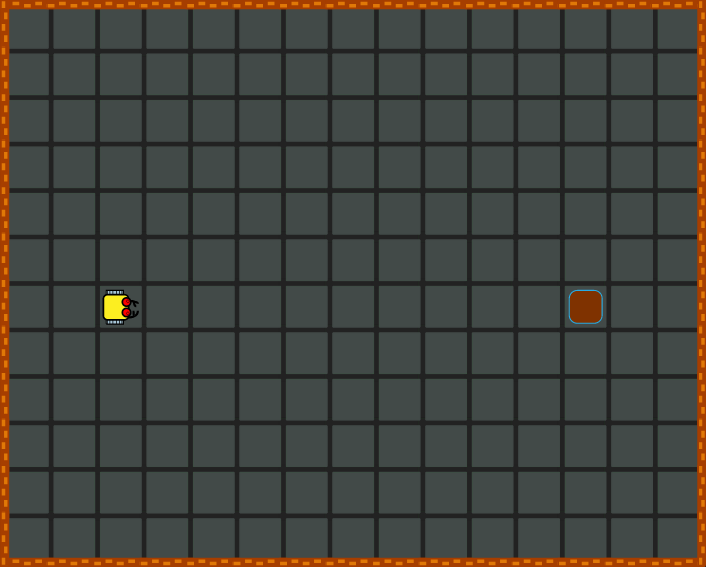
\includegraphics[height=0.4\textwidth]{img/c01.png}
\end{center}
\vspace{-4mm}
\caption{Karel gets home elegantly, using the {\tt repeat} command.}
\label{fig:c01}
\vspace{-4mm}
\end{figure}
\noindent


\subsection{Exercise C02 - Lucky Strike}

{\em Karel is about to find a pile of 12 gems! Write a program for the robot to collect the gems and get home. Use the {\tt repeat} command for any repeated action. 

\begin{figure}[!ht]
\begin{center}
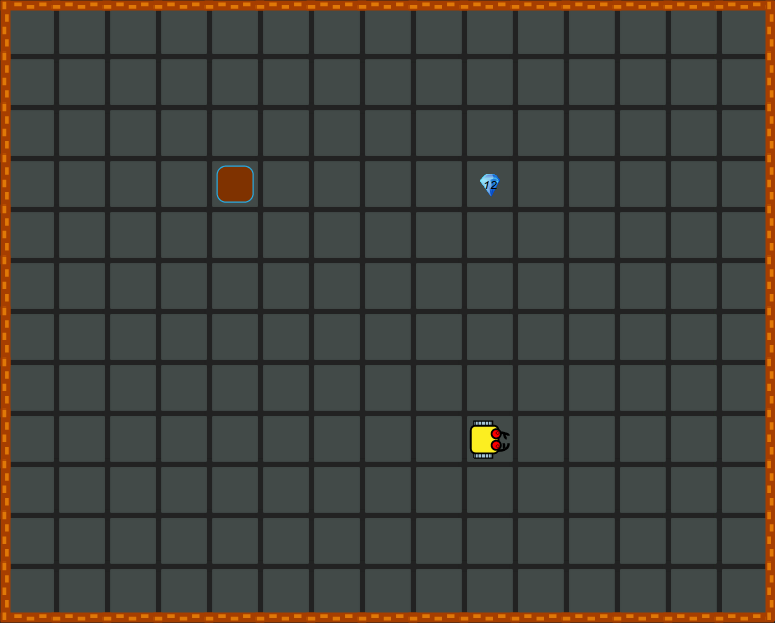
\includegraphics[height=0.4\textwidth]{img/c02.png}
\end{center}
\vspace{-4mm}
\caption{Karel is about to find a pile of 12 gems!}
\label{fig:c02}
\vspace{-4mm}
\end{figure}
\noindent

\newpage

\subsection{Exercise C03 - Feelin' Lucky}

{\em Karel is feeling lucky today. He wants to just step outside his house, 
turn around five times, then pick up one gem somewhere, and get back inside!}


\begin{figure}[!ht]
\begin{center}
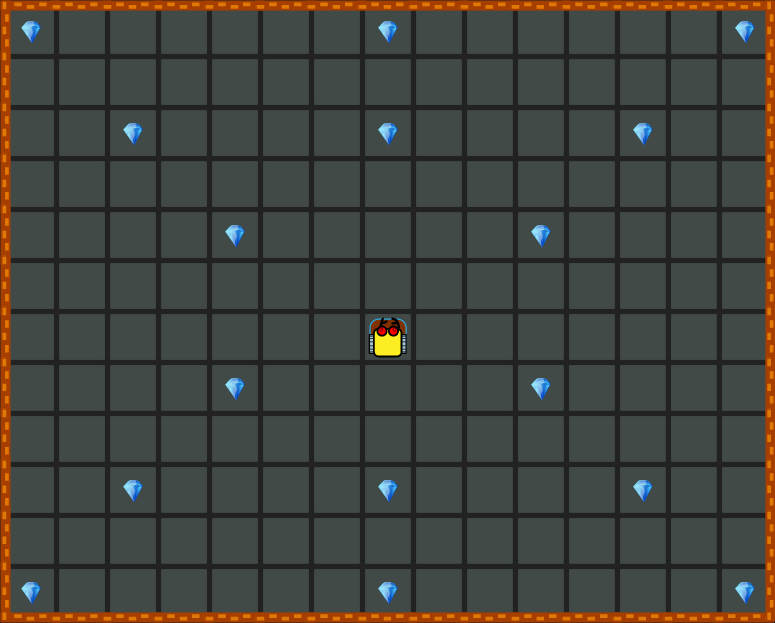
\includegraphics[height=0.4\textwidth]{img/c03.png}
\end{center}
\vspace{-4mm}
\caption{Karel is feeling lucky today.}
\label{fig:c03}
\vspace{-4mm}
\end{figure}
\noindent


\subsection{Exercise C04 - Garage Sale}

{\em Karel needs to sell 10 of his oldest gems in order to make space for new ones. 
Write a program for the robot to step out of his garage, put 10 gems on the ground, 
and then turn back and get back inside! Use the {\tt repeat} command for any repeated 
action.}


\begin{figure}[!ht]
\begin{center}
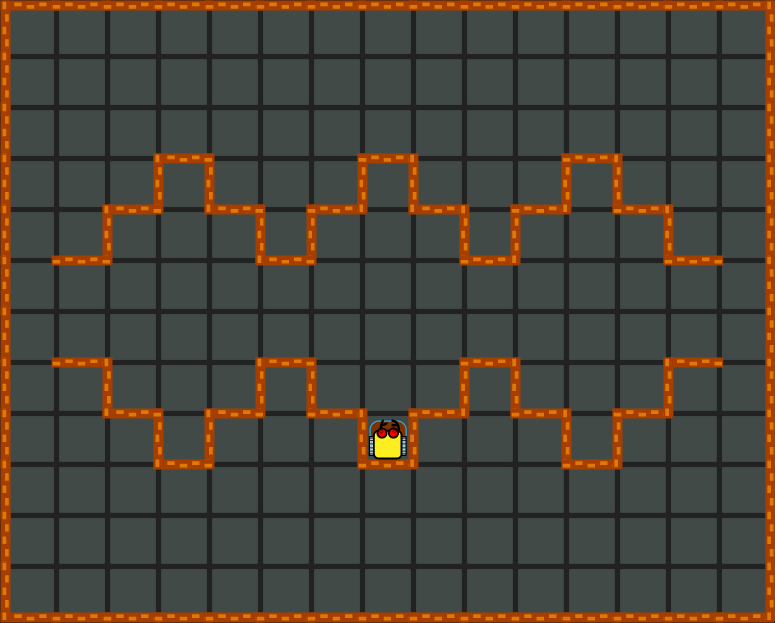
\includegraphics[height=0.4\textwidth]{img/c04.png}
\end{center}
\vspace{-4mm}
\caption{Karel is getting ready for garage sale.}
\label{fig:c04}
\vspace{-10mm}
\end{figure}
\noindent

\newpage

\subsection{Exercise C05 - String of Gems}

{\em Write a program for Karel to collect all nine gems and get home! 
Writing one command per line, your program should not have more 
than three lines.}.

\begin{figure}[!ht]
\begin{center}
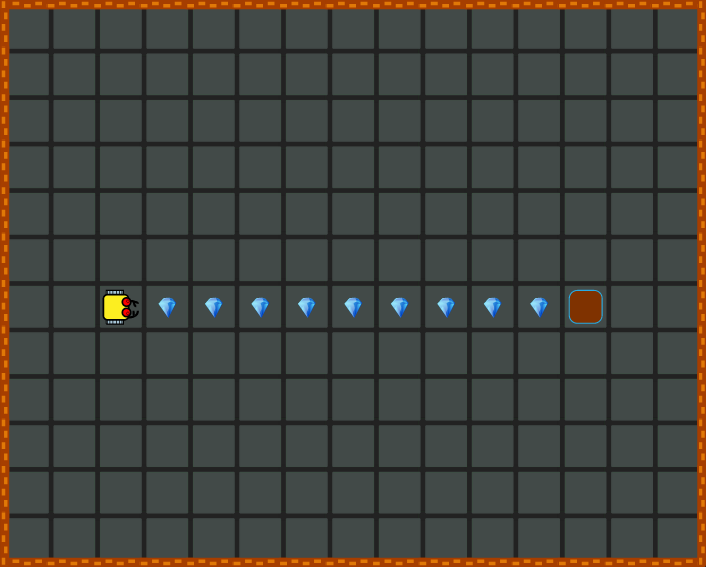
\includegraphics[height=0.4\textwidth]{img/c05.png}
\end{center}
\vspace{-4mm}
\caption{Nine gems are between Karel and his home.}
\label{fig:c05}
%\vspace{-10mm}
\end{figure}
\noindent

\section{Intermission - Working with Input and Text Cells} \label{sec:editmenu}

\subsection{Objectives} 
 
\begin{itemize}
\item Learn how to add descriptive text cells.
\item Learn when it makes sense to have multiple input cells and how to add them.
\item Learn how to run all input cells at once, and how to run them individually.
\item Learn how to clear, collapse, remove and merge cells.
\end{itemize}
It is a very good habit to add comments to programs (every line starting with the '{\tt \#}'
symbol is a comment) and also to include descriptive 
texts in Karel worksheets, since descriptions make it easier for someone else to 
understand your program. Sometimes you may be in the position of the "someone else" yourself,
when you return to your own program some time after you wrote it. Here are a couple of 
simple new rules to remember:
\begin{enumerate} 
\item New text cell can be added above or under the current cell via the option 
      {\em Add new text cell} in the Edit menu. 
      After an empty text cell appears, click into it and add text. The text can be 
      formatted using Restructured Text Format (RST). After your text is finished, click 
      on {\em save} under the text cell. 
\item The most commonly used formatting operations in RST are 
      \begin{itemize}
      \item Making some text bold face. For this, put a double asterisk '{\tt **}' on either 
      side of the text. For example, type {\tt **This is bold face**} in RST.
      \item Headings are obtained by undelining some text with the '{\tt =}' symbols.
      An example of a heading is:
\begin{verbatim}
This is a Heading
=================
\end{verbatim}
      \item The RST format is very popular and so it is easy to Google more information
      if needed.
      \end{itemize}
\item New input cell can be added by clicking on {\em add} (located under each input cell). 
      Having multiple input cells can be useful, for example, to test various versions 
      of your program, or if you want to run parts of your program separately. 
\item Clicking on {\em clear} under an input cell will erase its contents.
\item Any cell can be collapsed by clicking on the bracket located on its right side. Collapsed
      cells can be expanded by clicking on the blue button that appears when a cell is 
      collapsed.
\item Clicking on {\em remove} under an input cell will remove it. All text in that cell will be lost.
\item Run programs via the blue arrow button in the menu (this will evaluate all input
      cells). Each cell can be evaluated individually by clicking on {\em run} (located under 
      each input cell). If there is just one input cell, both options are equivalent.
\item Running programs can be stopped using the blue square button in the menu. 
\item If a particular
      input cell needs to be stopped, then use the {\em stop} button under that cell.
\end{enumerate}

\subsection{Review questions}

\begin{enumerate}
\item How can a new text cell be added?
\begin{enumerate}
\item[A1] By clicking on {\em add} under an existing input cell.
\item[A2] Through {\em Add new text cell} in the Edit menu.
\item[A3] Through {\em New} in File menu.
\item[A4] Through {\em Clone} in File menu.
\end{enumerate}
\item How can we add a new input cell?
\begin{enumerate}
\item[A1] By clicking on {\em add} under an existing input cell.
\item[A2] Through {\em Add new input cell} in the Edit menu.
\item[A3] Through {\em New} in File menu.
\item[A4] Through {\em Clone} in File menu.
\end{enumerate}
\item When should we have multiple input cells?
\begin{enumerate}
\item[A1] When our program contains more than one command.
\item[A2] When we want to run parts of the program separately.
\item[A3] When a command is repeated multiple times.
\item[A4] When the program is longer than 10 lines.
\end{enumerate}
\item What do we need to do in order to erase all text from an input cell?
\begin{enumerate}
\item[A1] Close Karel, logout from NCLab and login again. 
\item[A2] Restart Karel.
\item[A3] Remove the input cell and add a new one in its place.
\item[A4] Click on {\em clear} under the input cell.
\end{enumerate}
\item How can a cell be collapsed?
\begin{enumerate}
\item[A1] Click on {\em remove} under the input cell.
\item[A2] Through {\em Collapse} in File menu.
\item[A3] By clicking on the bracket on the right of the cell.
\item[A4] By clicking on {\em collapse} under the cell.
\end{enumerate}
\item How can an input cell be removed?
\begin{enumerate}
\item[A1] Click on {\em add} under the input cell.
\item[A2] Click on {\em remove} under the input cell.
\item[A3] Click on {\em clear} under the input cell.
\item[A4] Switch to Build mode and back.
\end{enumerate}
\item How can we evaluate all input cells at once?
\begin{enumerate}
\item[A1] Through {\em Expand all cells} in Edit menu.
\item[A2] Click on the blue square button.
\item[A3] Click on {\em run} under the last input cell.
\item[A4] Click on the blue arrow button.
\end{enumerate}
\item How should running programs be stopped?
\begin{enumerate}
\item[A1] Click on the blue arrow button.
\item[A2] Close the main Karel window.
\item[A3] Click on the blue square button.
\item[A4] Click on {\em stop} under the last input cell.
\end{enumerate}
\item How can we evaluate just one selected input cell?
\begin{enumerate}
\item[A1] Copy and paste the contents of all 
          input cells into the first one, and remove them.
\item[A2] Clicking on the blue arrow button in the menu. 
\item[A3] Clicking on {\em run} under the input cell.
\item[A4] Clicking on {\em remove} under the input cell.
\end{enumerate}
\end{enumerate}




\section{Section D - Conditions}

\subsection{Objectives} 

\begin{itemize}
\item Understand the function of Karel's five sensors.
\item Learn to use the sensors in conjunction with {\em conditions} to help Karel 
      check his surroundings and react accordingly. For example, you will learn to first 
      check whether wall is ahead before making a step forward, checking whether there
      is a gem on the ground before attempting to pick it up, etc.
\end{itemize}

\noindent
Karel has built-in sensors to better navigate in the maze:

\subsection{Karel's five sensors}

\noindent
\underline{{\tt wall} sensor}

The first one is an infrared sensor {\tt wall} that the robot uses to determine 
whether it is safe to make one step forward, or whether there is a wall. This is 
illustrated in Fig. \ref{fig:dede-ifelse}.

\begin{figure}[!ht]
\begin{center}
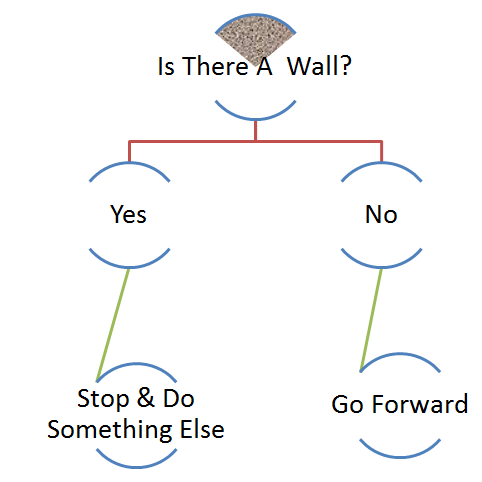
\includegraphics[height=0.4\textwidth]{img/salih-ifelse.png}
\end{center}
\vspace{-4mm}
\caption{This is how Karel uses the {\tt wall} sensor!}
\label{fig:dede-ifelse}
%\vspace{-10mm}
\end{figure}
\noindent
The usage of the {\tt wall} sensor in a program can be illustrated using a simple program "Careful step" 
where Karel first checks whether there is a wall ahead before
making a step. If there is wall, he turns back: 

\begin{verbatim}
# Program "Careful step".
if wall
  repeat 2
    left
else
  go
\end{verbatim}
As we mentioned before, the symbol '{\tt \#}' introduces a comment, meaning that the line 
of code behind it is ignored by the robot.
The {\tt else} branch does not have to be there if it is not needed. Notice the indentation 
of the bodies of the {\tt if} and {\tt else} branches - this is analogous 
to how we indent the body of the {\tt repeat} command.\\

\noindent
\underline{{\tt gem} sensor}

This sensor returns true if the robot stands on a gem, false otherwise. \\

\noindent
\underline{{\tt empty} sensor}

This sensor returns true if the robot's bag with gems is empty, false otherwise. \\

\noindent
\underline{{\tt north} sensor}

This sensor returns true if the robot is facing North, false otherwise.\\

\noindent
\underline{{\tt home} sensor}

This sensor returns true if the robot is at home, false otherwise.\\

\noindent
\underline{Testing opposites}

Karel can also use the reserved word {\tt not} to test the opposites.
For illustration, the previous program can be rewritten as follows, without changing its function:
\begin{verbatim}
# Program "Careful step".
if not wall
  go
else
  repeat 2
    left
\end{verbatim}

\subsection{Programming hints}

Good programmer is a careful programmer! Errors can be avoided by always checking the 
appropriate sensor before making an action. A few examples of careful actions:
 
\begin{verbatim}
if not wall
  go
\end{verbatim}
Another example:
 
\begin{verbatim}
if gem
  get
\end{verbatim}
And a last one:
 
\begin{verbatim}
if not empty
  put
\end{verbatim}

\subsection{Review questions}

\begin{enumerate}
\item When does the {\tt gem} sensor check true?
\begin{enumerate}
\item[A1] There is at least one gem in the maze.
\item[A2] There is at least one gem in front of the robot.
\item[A3] There are one or more gems under the robot.
\item[A4] The robot's bag contains at least one gem.
\end{enumerate}
\item When does the {\tt North} sensor check true?
\begin{enumerate}
\item[A1] The robot's home is North of him.
\item[A2] The robot is North of his home.
\item[A3] The robot faces South.
\item[A4] The robot faces North.
\end{enumerate}
\item When does the {\tt empty} sensor check true?
\begin{enumerate}
\item[A1] The robot's bag is empty.
\item[A2] There are no gems where the robot stands.
\item[A3] There are no gems in the maze.
\item[A4] There are not gems in the robot's home.
\end{enumerate}
\item When does the {\tt home} sensor check true?
\begin{enumerate}
\item[A1] Robot's home is right in front of the robot.
\item[A2] The robot is in his home.
\item[A3] Robot's home is straight ahead of the robot.
\item[A4] The robot needs to go home to drop all gems that he collected.
\end{enumerate}
\item When does the {\tt wall} sensor check true?
\begin{enumerate}
\item[A1] The robot will reach a wall with one or more steps. 
\item[A2] There is a wall on the robot's right-hand side.
\item[A3] There is a wall right in front of the robot.
\item[A4] There is a wall on the robot's left-hand side.
\end{enumerate}
\item When can Karel see from where he stands whether a wall is two steps ahead?
\begin{enumerate}
\item[A1] Never.
\item[A2] If his home is not in the way.
\item[A3] If no gem is in the way.
\item[A4] If no other wall is in the way.
\end{enumerate}
\item When can the robot check without turning whether a wall is on his right?
\begin{enumerate}
\item[A1] Any time, there is the sensor {\tt right} for that.
\item[A2] Any time, there is the sensor {\tt wall} for that.
\item[A3] Only if he is not at home.
\item[A4] Never.
\end{enumerate}
\item Can Karel check from where he stands whether a gem is one step away?
\begin{enumerate}
\item[A1] Yes, there is the sensor {\tt gem} for that.
\item[A2] No.
\item[A3] Yes but the gem must be in front of him.
\item[A4] Yes but not when he is at home.
\end{enumerate}
\item Can he check from where he stands whether his home is one step away?
\begin{enumerate}
\item[A1] Yes but his home must be in front of him.
\item[A2] Yes, there is the sensor {\tt home} for that.
\item[A3] No.
\item[A4] Yes but not when he is at home.
\end{enumerate}
\item Can the robot check whether he has at least one gem in the bag?
\begin{enumerate}
\item[A1] No.
\item[A2] Yes, he can use the {\tt gem} sensor. 
\item[A3] No, the sensor gem only works for one gem.
\item[A4] Yes, he can use the {\tt empty} sensor.
\end{enumerate}
\item Which program makes Karel check whether he stands on a gem, and if so, to pick it up.
\begin{enumerate}
\item[A1] 
\begin{verbatim}
if gem
  get
\end{verbatim}
\item[A2] 
\begin{verbatim}
if not empty
  get
\end{verbatim}
\item[A3] 
\begin{verbatim}
if get
  gem
\end{verbatim}
\item[A4] 
\begin{verbatim}
if empty
  get
\end{verbatim}
\end{enumerate}
\item Which program will turn Karel always to the North?
\begin{enumerate}
\item[A1] 
\begin{verbatim}
repeat 4
  if not north 
    left
\end{verbatim}
\item[A2] 
\begin{verbatim}
if not north 
  left
else 
  right
\end{verbatim}
\item[A3] 
\begin{verbatim}
if south
  repeat 2
    right
\end{verbatim}
\item[A4] 
\begin{verbatim}
if not north 
  right
\end{verbatim}\end{enumerate}

\end{enumerate}

\subsection{Exercise D01 - In the Fog}

{\em Several gems lie on the ground between the robot and his home which is 10 steps away. 
He cannot see where the gems are though. 
Write a program for Karel to collect all gems and get home. With one command per 
line, your program should have at most 4 lines.}


\begin{figure}[!ht]
\begin{center}
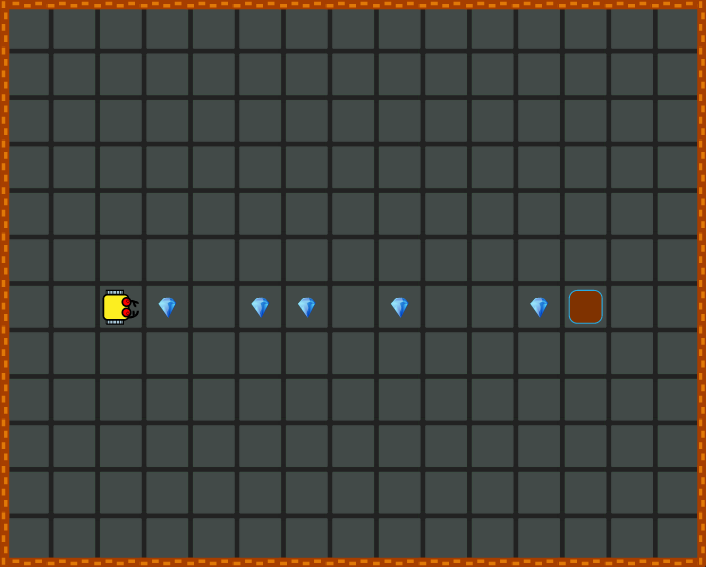
\includegraphics[height=0.4\textwidth]{img/d01.png}
\end{center}
\vspace{-4mm}
\caption{Several gems are at random positions between the robot and his home.}
\label{fig:d01}
\vspace{-4mm}
\end{figure}
\noindent

\subsection{Exercise D02 - Stony Meadows}

{\em Karel is walking on a meadows that is covered with irregularly 
scattered stones. Write a program for the robot to get to his home, 
avoiding stones, and collecting all gems!  }


\begin{figure}[!ht]
\begin{center}
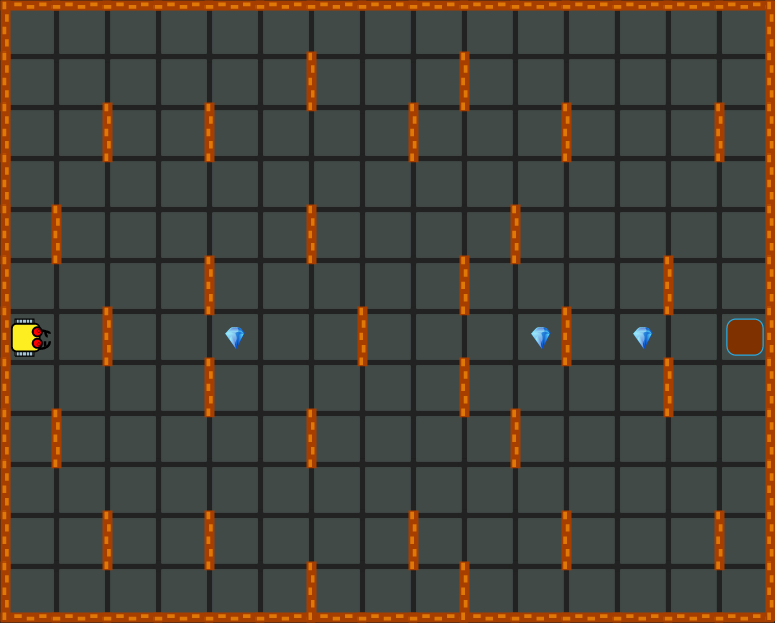
\includegraphics[height=0.4\textwidth]{img/d02.png}
\end{center}
\vspace{-4mm}
\caption{Karel is crossing a stony meadows.}
\label{fig:d02}
\vspace{-10mm}
\end{figure}
\noindent

\newpage




\subsection{Exercise D03 - Filling the Blanks}

{\em Karel stores all his gems in a secret chest in his cellar. 
Currently, some shelves are empty. Write a program for Karel to 
inspect all shelves and put a gem where one is missing! After that, he needs to get 
home as usual. With one 
command per line, your program should have at most 7 lines.}

\begin{figure}[!ht]
\begin{center}
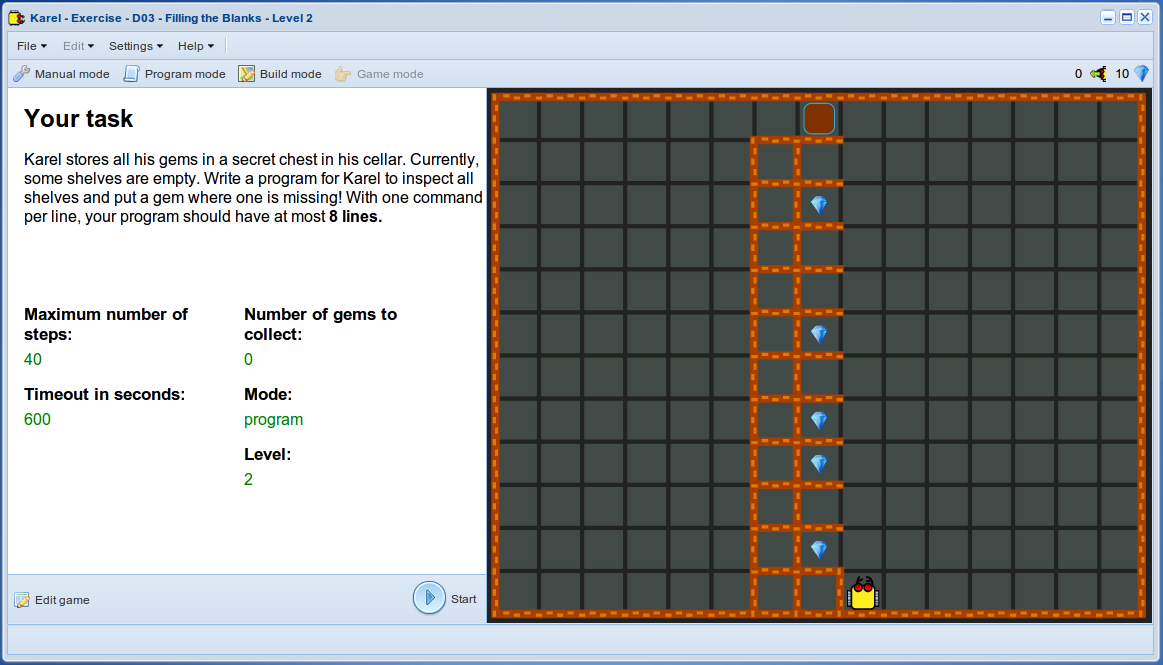
\includegraphics[height=0.4\textwidth]{img/d03.png}
\end{center}
\vspace{-4mm}
\caption{Filling empty shelves with gems.}
\label{fig:d03}
\vspace{-4mm}
\end{figure}
\noindent



\section{Section E - Conditional Loop}

\subsection{Objectives} 
 
\begin{itemize}
\item Learn to repeat a command or a sequence of commands when it is not known 
      how many repetitions will be needed.
\end{itemize}

\subsection{The {\tt while} command}

Often Karel needs to repeat something, {\em not knowing in advance how many repetitions
there will be}. So, the {\tt repeat} command is not practical. This can be the case, for example, 
when the robot is asked to walk straight ahead until he reaches the closest wall.
Remember that he only can see walls that are right ahead of him -- walls 
that are further away he can't see. Such a program would be:

\begin{verbatim}
while not wall
  go
\end{verbatim}
Or, Karel may be asked to walk until he gets home:

\begin{verbatim}
while not home
  go
\end{verbatim}
Beware though -- {\bf this program is dangerous} since the robot will crash into a wall
if his home is not straight ahead of him!

Another example: The robot may be asked to empty his bag (he does not know how many gems are in it): 
 
\begin{verbatim}
while not empty
  put
\end{verbatim}
Or, he may be asked to collect all gems from a pile (he does not know 
how many gems there are):

\begin{verbatim}
while gem
  get
\end{verbatim}
Or we may ask him to turn to face North (he does not know which direction he is
facing):

\begin{verbatim}
while not north
  left
\end{verbatim}
At last, let us face the following situation: Karel is asked to 
turn South, walk straight ahead until he reaches the closest wall, and 
collect all gems that he can find on the way:

\begin{verbatim}
# First turn North.
while not north
  left

# Then turn South.
repeat 2
  left

# Go straight ahead and pick all gems.
while not wall
  if gem
    get
  go

# Pick gem at the wall (if any).
if gem
  get
\end{verbatim}
Notice that we first need to turn the robot to face North -- this is because North 
is the only direction that he can check!

\subsection{Review questions}

\begin{enumerate}
\item What is the difference between the {\tt repeat} and {\tt while} loops?
\begin{enumerate}
\item[A1] Body of the {\tt while} loop does not have to be indented.
\item[A2] The {\tt while} loop only can be used when the number of repetitions is known a priori.
\item[A3] The {\tt repeat} loop can do 100 repetitions maximum.
\item[A4] The {\tt repeat} loop only can be used when the number of repetitions is known a priori.
\end{enumerate}
\item Which program will always turn Karel to face West?
\begin{enumerate}
\item[A1] 
\begin{verbatim}
repeat 4
  left
\end{verbatim}
\item[A2] 
\begin{verbatim}
while not west
  right
\end{verbatim}
\item[A3] 
\begin{verbatim}
while not north
  left
left
\end{verbatim}
\item[A4] 
\begin{verbatim}
while not north 
  right
right
\end{verbatim}
\end{enumerate}
\item The maze does not contain any gems and any walls except for the ones that form the outer rectangular boundary.
      The robot stands in the south-west corner facing East. Which program will make the robot walk along the 
      boundary of the maze and bring him back to the original position?
\begin{enumerate}
\item[A1] 
\begin{verbatim}
repeat 4
  while not wall
    go
\end{verbatim}
\item[A2] 
\begin{verbatim}
repeat 4
  while not wall
    go
  left
\end{verbatim}
\item[A3] 
\begin{verbatim}
repeat 4
  while not wall
    go
  right
\end{verbatim}
\item[A4] 
\begin{verbatim}
repeat 4
  while not wall
    left
  go
\end{verbatim}
\end{enumerate}
\end{enumerate}

\subsection{Exercise E01 - South West}

{\em Karel is somewhere in the maze, facing a random direction. Write a program for the robot to get 
to his home which is in the south-west corner!}\\[-7mm]


\begin{figure}[!ht]
\begin{center}
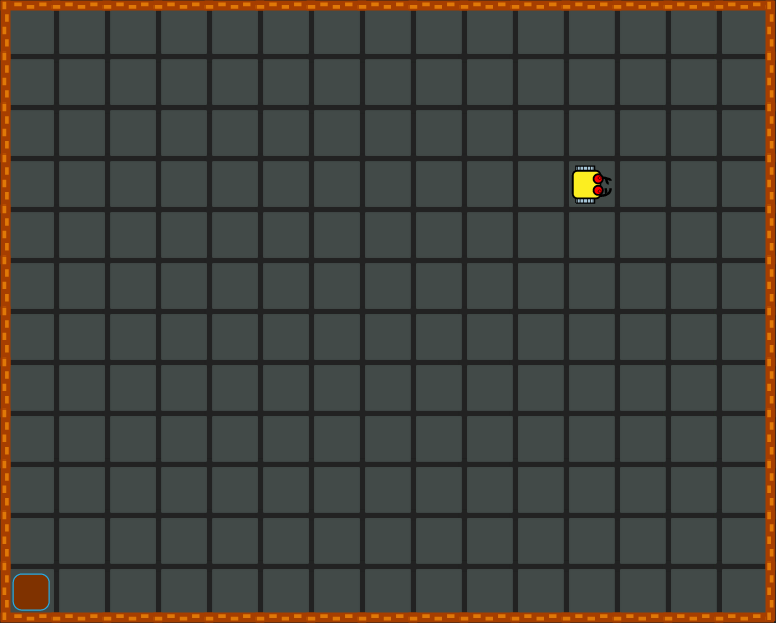
\includegraphics[height=0.4\textwidth]{img/e01.png}
\end{center}
\vspace{-4mm}
\caption{Karel only knows that his home is in the SW corner of the maze.}
\label{fig:e01}
%\vspace{-12mm}
\end{figure}
\noindent


\subsection{Exercise E02 - Hide-and-Seek}

{\em Karel's friends are hiding. To find them, he has to straight ahead 
and whenever he finds a gem, he has to collect it, 
turn left, and keep walking. Eventually, they said, he will get to the place 
where they are. Write a program for Karel to find his friends!}\\[-7mm]


\begin{figure}[!ht]
\begin{center}
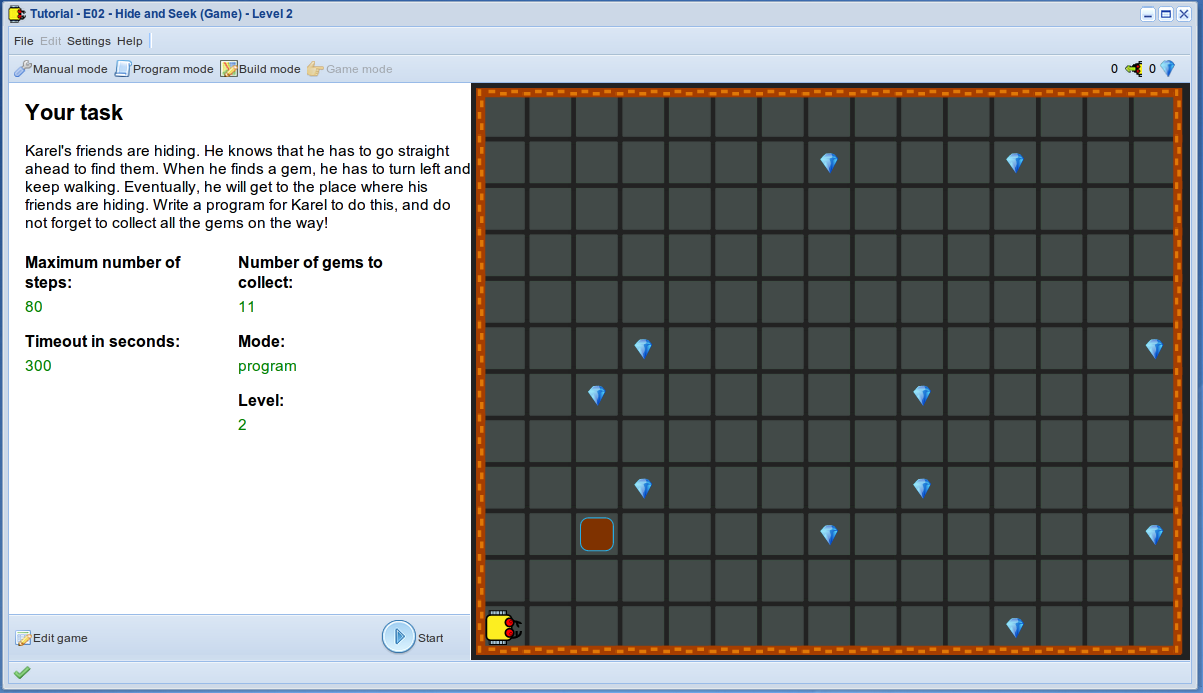
\includegraphics[height=0.4\textwidth]{img/e02.png}
\end{center}
\vspace{-4mm}
\caption{Karel plays hide-and-seek with his friends.}
\label{fig:e02}
\vspace{-10mm}
\end{figure}
\noindent
\newpage

\subsection{Exercise E03 - Walk the Line}

{\em Karel stands next to a straight wall and he knows that his home is somewhere on the other side of it. He does not know how long the wall is, nor the exact position of his home. Write a program for the robot to get there!}

\begin{figure}[!ht]
\begin{center}
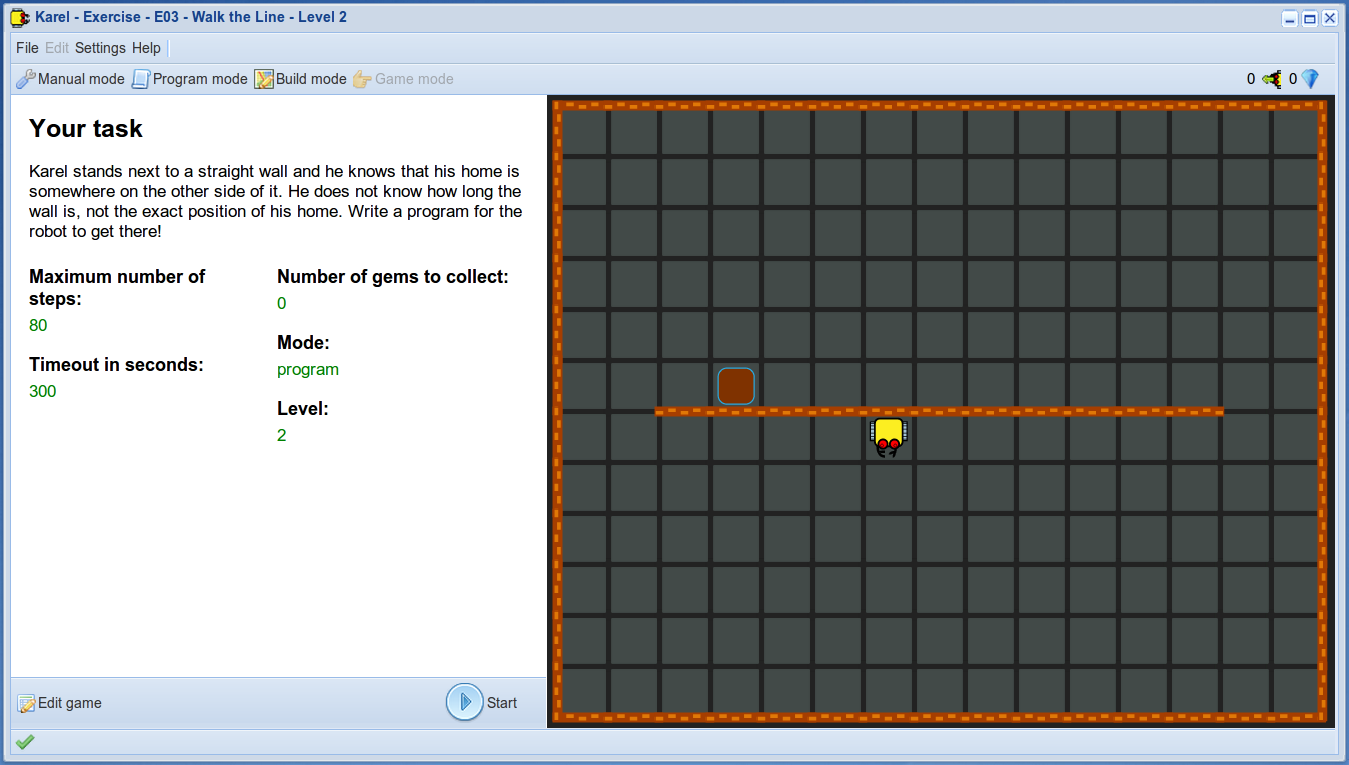
\includegraphics[height=0.4\textwidth]{img/e03.png}
\end{center}
\vspace{-4mm}
\caption{Karel only knows that his home is on the other side of the wall.}
\label{fig:e03}
%\vspace{-10mm}
\end{figure}
\noindent


\section{Section F - Defining New Commands} \label{sec:newcom}

\subsection{Objectives} 
 
\begin{itemize}
\item Learn that replicating computer code is a very bad habit.
\item Learn that splitting the big task into smaller ones will simplify the solution a lot. 
\item Learn to bring more structure and clarity into your programs by introducing new commands.
\end{itemize}

\subsection{Programming hints}

{\em Always look for small tasks that can be solved independently of the big ones.
Solve the small tasks first, and you'll see that the big ones get much simpler. The 
importance of what we just said cannot be stressed more. Please read these three 
lines once more.}

\newpage
\noindent
The fact that you are reading this line of text proves that you are not 
a perfect programmer yet. Otherwise you would be stuck forever in the 
previous three lines that form an infinite loop!

\begin{figure}[!ht]
\begin{center}

\includegraphics[width=0.3\textwidth]{img/smiley.png}
\end{center}
\vspace{-1cm}
\end{figure}

\subsection{Never replicate code in a program!}

A new command should be defined whenever it becomes clear that the same 
action is repeated in the algorithm multiple times (yes, we talk about the algorithm,
not about the program). If you start writing a program and then realize that the same
code repeats itself at various places, then probably you did not do a good job 
designing the algorithm.

Sometimes it might be 
tempting to just replicate the same code several times in the 
program, because it does the same thing, but do not do it! This would be very bad programming
and sooner or later your own code would punish you for that. 
You would make a small change at one place but forget to do it 
in all the other places. Then your code would start 
acting strange, it would sometimes work and sometimes fail. 
You would spend lots of time looking for the mistakes, find some 
of them but not all, and your program would become unreliable
and after some time irreparable. You would find that you need to 
rewrite it from scratch.

\subsection{Defining new commands}

New commands are defined using the reserved word 
{\tt def}. For example, in a program where the robot needs to turn back
many times, it is a good idea to define a new command {\tt back}
as follows:

\begin{verbatim}
def back
  repeat 2
    left
\end{verbatim}
Note the indent -- the body of a new command needs to be indented 
analogously to the bodies of loops and conditions.

\subsection{Revisiting exercise A07}

Let us return to the exercise A07 - Right Button for a moment.
A really bad program to solve this task would be:

{\small
\begin{verbatim}
right
go
go
go
go 
get
right
go
go
go
go 
get
right
go
go
go
go
get
\end{verbatim}
}
\noindent
Can you see how many times the same code is repeated?! In order to fix this, 
we should define new command {\tt foursteps} as
follows:

{\small
\begin{verbatim}
def foursteps
  repeat 4
    go
\end{verbatim}
}
\noindent
With this new command, the above code simplifies to 

{\small
\begin{verbatim}
right
foursteps
get
right
foursteps
get
right
foursteps
get
\end{verbatim}
}
\noindent
There are still repetitions that must be eliminated! So we define a new command 
{\tt walkedge}:

{\small
\begin{verbatim}
def walkedge
  right
  foursteps
  get
\end{verbatim}
}
\noindent
Now with the new commands {\tt foursteps} and
{\tt walkedge}, our program simplifies to:

{\small
\begin{verbatim}
while not home
  walkedge
\end{verbatim}
}
\noindent
It is the task of the first exercise in this Section to implement this program. But before we 
do so, let us mention one very important thing.

\subsection{Solution procedure revisited (and corrected)}

Let's forget the commands that we defined above.
Experienced programmer would never approach the problem the way we did.
He (or she but let's use "he" for simplicity) 
would first look at the problem, trying to recognize repeating patterns. 
He would find that the task can be fulfilled by repeating one simpler task 
three times. So, without knowing exactly how the smaller task is going to 
be solved, he would write:

{\small
\begin{verbatim}
while not home
  walkedge
\end{verbatim}
}
\noindent
Next he would define the new command {\tt walkedge} as follows:

{\small
\begin{verbatim}
def walkedge
  right
  foursteps
  get
\end{verbatim}
}
\noindent
He would not bother defining the command 
{\tt foursteps} yet, because he knows that this will be 
simple. And as the last step, to make the program work, he would 
define:

{\small
\begin{verbatim}
def foursteps
  repeat 4
    go
\end{verbatim}
}

\subsection{Review questions}

\begin{enumerate}
\item Should we, or should we not always try to split a big task into smaller ones?
\begin{enumerate}
\item[A1] No, because the resulting program would be too long.
\item[A2] Yes, because then we can only solve those ones that we like.
\item[A3] Yes, because then we can ask friends to solve some of them for us.
\item[A4] Yes, because the big task becomes simpler to solve.
\end{enumerate}
\item Should we, or should we not replicate computer code?
\begin{enumerate}
\item[A1] Yes, because the resulting program is faster.
\item[A2] Yes, because we do not have to think about new commands.
\item[A3] No, because our code would become prone to errors.
\item[A4] No, because the Karel language does not allow that.
\end{enumerate}
\item When should a new command be defined?
\begin{enumerate}
\item[A1] Whenever the same command is repeated on two consecutive lines in the code.
\item[A2] Whenever the algorithm contains an action that is repeated multiple times
          (a small task inside a big one).
\item[A3] Whenever the code contains an {\tt if - else} statement.
\item[A4] If the code is longer than 100 lines.
\end{enumerate}
\item Which command will empty the robot's bag without causing an error?
\begin{enumerate}
\item[A1] 
\begin{verbatim}
def emptybag
  while gem
    put
\end{verbatim}
\item[A2] 
\begin{verbatim}
def emptybag
  while not gem
    put
\end{verbatim}
\item[A3] 
\begin{verbatim}
def emptybag
  while empty
    put
\end{verbatim}
\item[A4] 
\begin{verbatim}
def emptybag
  while not empty
    put
\end{verbatim}
\end{enumerate}
\item Which command will turn Karel to the South no matter 
      which direction he faces initially?
\begin{enumerate}
\item[A1] 
\begin{verbatim}
def turnsouth
  while north
    repeat 2
      left
\end{verbatim}
\item[A2] 
\begin{verbatim}
def turnsouth
  while not north
    repeat 2
      left
\end{verbatim}
\item[A3] 
\begin{verbatim}
def turnsouth
  while not north
    repeat 3
      left
\end{verbatim}
\item[A4] 
\begin{verbatim}
def turnsouth
  while not north
    left
  repeat 2
    left
\end{verbatim}
\end{enumerate}
\end{enumerate}

\newpage
\subsection{Exercise F01 - Four Star Hotel}

{\em Before getting home, Karel has to collect all four stars of gems!}


\begin{figure}[!ht]
\begin{center}
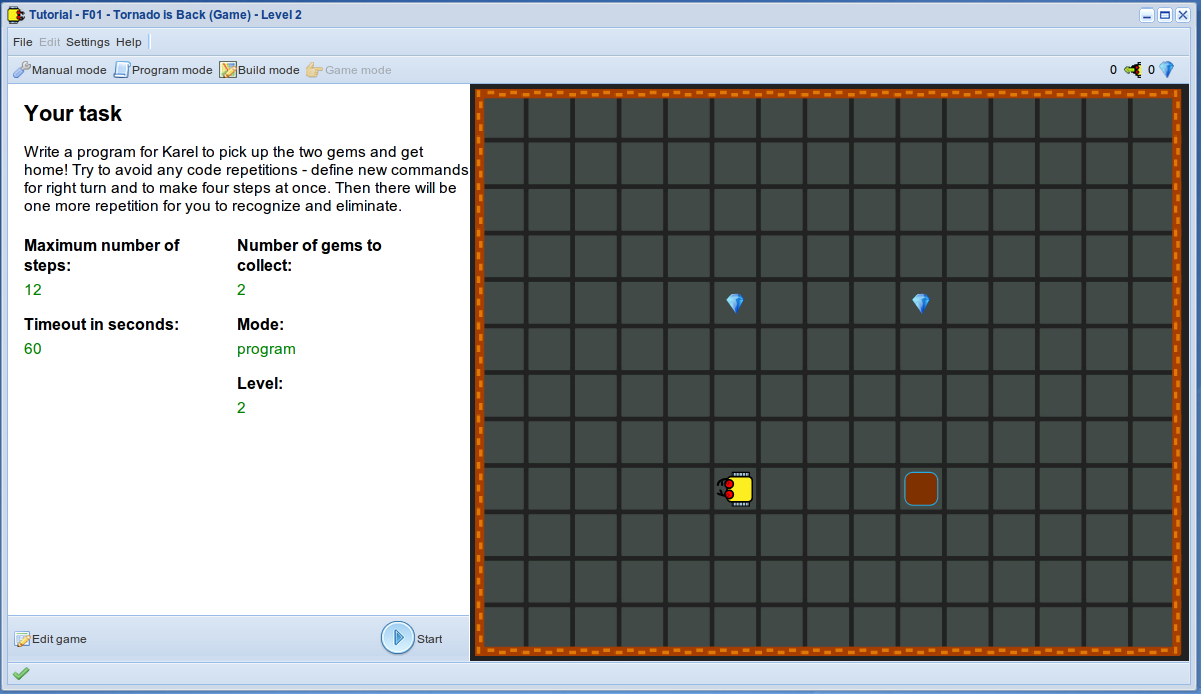
\includegraphics[height=0.4\textwidth]{img/f01.png}
\end{center}
\vspace{-4mm}
\caption{Karel needs to collect four stars of gems.}
\label{fig:f01}
\vspace{-10mm}
\end{figure}
\noindent

\subsection{Exercise F02 - U-Haul}

{\em Write a program for the robot to move the 6x6 square of gems to the opposite corner of the maze. The task is finished when the robot is back home.}

\begin{figure}[!ht]
\begin{center}
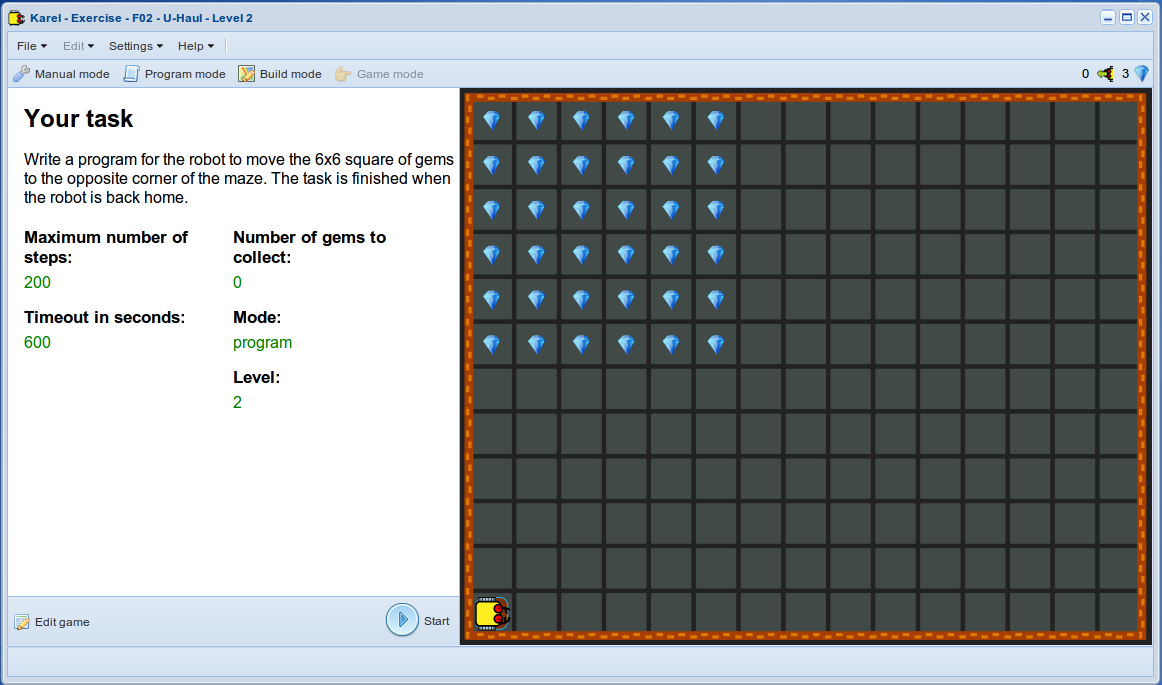
\includegraphics[height=0.4\textwidth]{img/f02.png}
\end{center}
\vspace{-4mm}
\caption{Karel needs to move the gems to the opposite corner of the maze.}
\label{fig:f02}
\vspace{-10mm}
\end{figure}
\noindent
\newpage

\subsection{\ \ Exercise F03 - Egg Hunt}

{\em Write a program for Karel to search all cells and collect all eggs (gems) that he can find. The task is finished when the robot is back home.}


\begin{figure}[!ht]
\begin{center}
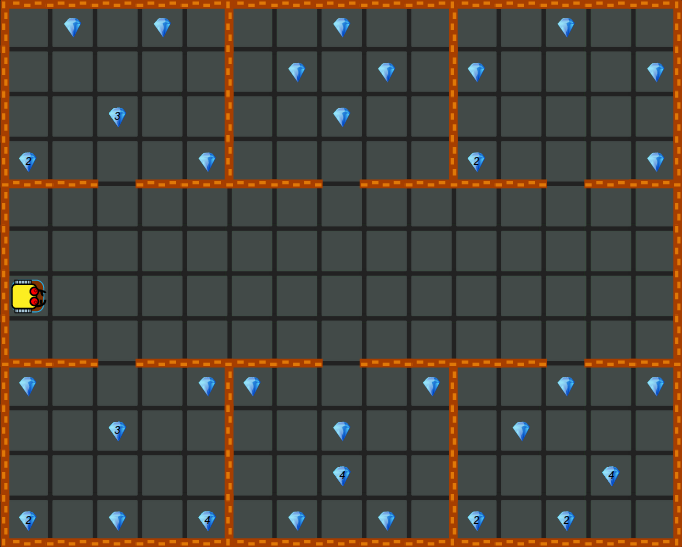
\includegraphics[height=0.4\textwidth]{img/f03.png}
\end{center}
\vspace{-4mm}
\caption{Easter is here, Karel is on egg hunt!}
\label{fig:f03}
\vspace{-10mm}
\end{figure}
\noindent

\subsection{\ \ Exercise F04 - Blind Carpenter}

{\em Karel is a blind carpenter who needs to install windows (gems) into a newly built house. All he knows is that the house is a rectangle and that each window is exactly one tile large, But he can't see where the openings for the windows are. Install the windows and return home!}


\begin{figure}[!ht]
\begin{center}
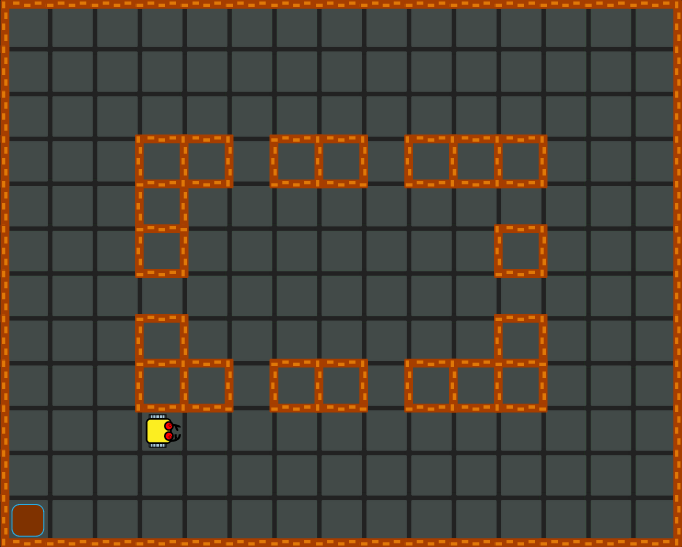
\includegraphics[height=0.4\textwidth]{img/f04.png}
\end{center}
\vspace{-4mm}
\caption{This time Karel installs windows.}
\label{fig:f04}
\vspace{-10mm}
\end{figure}
\noindent
\newpage


\subsection{\ \ Exercise F05 - Pirate Ship}

{\em Karel is on a pirate ship! Write a program for him to collect all 
gems and run away (to his home) before the pirates are back. Here Karel 
needs to be extremely efficient to survive. Therefore, there should be 
no repeating parts whatsoever in your program!}


\begin{figure}[!ht]
\begin{center}
\includegraphics[height=0.4\textwidth]{img/f05.png}
\end{center}
\vspace{-4mm}
\caption{Karel found a pirate treasure.}
\label{fig:f05}
\vspace{-10mm}
\end{figure}
\noindent

\subsection{\ \ Exercise F06 - Diamond Staircase}

{\em Write a program for Karel to climb the stairs, collect all gems, and get home!}


\begin{figure}[!ht]
\begin{center}
\includegraphics[height=0.4\textwidth]{img/f06.png}
\end{center}
\vspace{-4mm}
\caption{This time Karel has to do some climbing.}
\label{fig:f06}
\vspace{-10mm}
\end{figure}
\noindent
\newpage


\subsection{\ \ Exercise F07 - Plucking Flowers}

{\em Write a program for Karel to pluck all flowers that grow at the fence of his garden (gems), and get back home! Note two levels of repetition.}\\[-7mm]


\begin{figure}[!ht]
\begin{center}
\includegraphics[height=0.4\textwidth]{img/f07.png}
\end{center}
\vspace{-4mm}
\caption{Karel is plucking flowers along his fence.}
\label{fig:f07}
\vspace{-4mm}
\end{figure}
\noindent

\subsection{\ \ Exercise F08 - Gems for Friends}

{\em Karel has three gems in his bag, that he wants to give to his three friends R2, D2 and Marvin who live close by. Write a program for Karel to put a gem on the ground in the middle of each friend's home, and then return to his own home.}\\[-7mm]


\begin{figure}[!ht]
\begin{center}
\includegraphics[height=0.4\textwidth]{img/f08.png}
\end{center}
\vspace{-4mm}
\caption{Karel is going to give gems to his three friends R2, D2 and Marvin.}
\label{fig:f08}
\vspace{-10mm}
\end{figure}
\noindent
\newpage

\subsection{\ \ Exercise F09 - Diamond Rectangle}

{\em Karel stands in front of a rectangle with unknown dimensions. He knows that the rectangle is surrounded with gems. Write a program for the robot to walk around the rectangle, collect all gems, and get home!}\\[-7mm]


\begin{figure}[!ht]
\begin{center}
\includegraphics[height=0.4\textwidth]{img/f09.png}
\end{center}
\vspace{-4mm}
\caption{This time Karel does not know the size of the rectangle.}
\label{fig:f09}
\vspace{-10mm}
\end{figure}
\noindent

\subsection{\ \ Exercise F10 - Gem Jam!}

{\em In this maze, gems are distributed randomly along the walls. Otherwise 
the maze is empty. Karel's home is in the south-west corner, and the robot 
stands on the right of it, facing east. Write a program for Karel to collect 
all the gems and return home!}\\[-7mm]

\begin{figure}[!ht]
\begin{center}
\includegraphics[height=0.4\textwidth]{img/f10.png}
\end{center}
\vspace{-4mm}
\caption{Gem Jam!}
\label{fig:f10}
\vspace{-10mm}
\end{figure}
\noindent

\newpage

\subsection{\ \ Exercise F11 - The Matrix}

{\em Write a program for Karel to collect all gems and get back home! The record is 
210 steps made. Can you do it with fewer steps?}\\[-7mm]

\begin{figure}[!ht]
\begin{center}
\includegraphics[height=0.4\textwidth]{img/f11.png}
\end{center}
\vspace{-4mm}
\caption{The Matrix.}
\label{fig:f11}
\vspace{-10mm}
\end{figure}
\noindent

\subsection{\ \ Exercise F12 - Escape from Alcatraz}

{\em Karel is escaping from the Alcatraz prison! At the moment he is in an underground labyrinth with many random tunnels but only one of them leads to his freedom. Use the right-hand rule to find your way out!}\\[-7mm]


\begin{figure}[!ht]
\begin{center}
\includegraphics[height=0.4\textwidth]{img/f12.png}
\end{center}
\vspace{-4mm}
\caption{Karel is escaping from the Alcatraz prison.}
\label{fig:f12}
\vspace{-10mm}
\end{figure}
\noindent
\newpage

\subsection{\ \ Exercise F13 - Border Patrol}

{\em Write a program for Karel to check the perimeter of the maze using the 
right-hand rule. Do not forget to pick up all gems that you find on the way.}\\[-7mm]

\begin{figure}[!ht]
\begin{center}
\includegraphics[height=0.4\textwidth]{img/f13.png}
\end{center}
\vspace{-4mm}
\caption{Border Patrol.}
\label{fig:f13}
\vspace{-12mm}
\end{figure}
\noindent

\subsection{\ \ Exercise F14 - Ariadne's Thread}

{\em In an ancient Greek legend, princess Ariadne saved the life of her 
beloved Theseus by giving him a thread that he used to avoid getting lost 
in the maze of king Minos and kill a feared beast Minotaurus. Karel uses 
a similar technique - he leaves behind him a chain of gems that helps him 
to safely find his way back home. Your program needs to work for an 
arbitrary maze. You can assume that the string of gems is continuous 
and that it does not contain any loops.}\\[-7mm]

\begin{figure}[!ht]
\begin{center}
\includegraphics[height=0.4\textwidth]{img/f14.png}
\end{center}
\vspace{-4mm}
\caption{Maze of king Minos, home of the beast Minotaurus.}
\label{fig:f14}
\vspace{-10mm}
\end{figure}
\noindent

\newpage

\section{Section G - Recursion}

\subsection{Objectives} 
 
\begin{itemize}
\item Understand what recursion is and when it is advantageous to use it.
\item Learn to write good recursive algorithms.
\end{itemize}
By {\em recursion} we mean that an algorithm makes use of its own functionality. On program level,
this means that some command calls itself, either directly or through other commands.

\subsection{How it works} 

Consider the following program:
\begin{verbatim}
def reach_wall
  if not wall
    go
    reach_wall

reach_wall
\end{verbatim}
Imagine that the initial position of the robot is like in Fig. \ref{fig:rec1}.

\begin{figure}[!ht]
\begin{center}
\includegraphics[width=6cm]{img/rec-1.png}
\end{center}
\vspace{-4mm}
\caption{Robot's initial position.}
\label{fig:rec1}
\vspace{-4mm}
\end{figure}
\noindent
When the command {\tt reach\_wall} is first called, the robot stands three steps away from the wall and 
thus the {\tt if not wall} condition passes. Then the command {\tt go} follows and the robot's 
position changes as shown in Fig. \ref{fig:rec2}. 

\begin{figure}[!ht]
\begin{center}
\includegraphics[width=6cm]{img/rec-2.png}
\end{center}
\vspace{-4mm}
\caption{Robot's position after the first {\tt if not wall} condition passes and he makes the first step forward.}
\label{fig:rec2}
\vspace{-10mm}
\end{figure}
\newpage
\noindent
Next the robot executes the {\tt reach\_wall} command that follows the {\tt go} command. A good way to 
understand what happens is to imagine that the command is replaced with its own body. The corresponding 
program would look as follows:

\begin{verbatim}
if not wall
  go
  if not wall
    go
    reach_wall
\end{verbatim}
\noindent
Since the robot is two steps away from the wall, the second {\tt if not wall} condition passes and 
he makes a second step forward. His new position is shown in Fig. \ref{fig:rec3}.

\begin{figure}[!ht]
\begin{center}
\includegraphics[width=6cm]{img/rec-3.png}
\end{center}
\vspace{-4mm}
\caption{Robot's position after the second {\tt if not wall} condition passes and he makes a second step forward.}
\label{fig:rec3}
%\vspace{-10mm}
\end{figure}
\noindent
Next the robot executes the third {\tt reach\_wall} command. Again we can imagine that the command 
is replaced with its own body. The corresponding program would look as follows:

\begin{verbatim}
if not wall
  go
  if not wall
    go
    if not wall
      go
      reach_wall
\end{verbatim}
\noindent
Since the robot is one step away from the wall, the third {\tt if not wall} condition passes and 
he makes a third step forward. His new position is shown in Fig. \ref{fig:rec4}.

\newpage
\begin{figure}[!ht]
\begin{center}
\includegraphics[width=6cm]{img/rec-4.png}
\end{center}
\vspace{-4mm}
\caption{Robot's position after the third {\tt if not wall} condition passes and he makes a third step forward.}
\label{fig:rec4}
%\vspace{-10mm}
\end{figure}
\noindent
Next the robot executes the {\tt reach\_wall} command again and we can imagine that the command 
is replaced with its own body. The corresponding program would look as follows:

\begin{verbatim}
if not wall
  go
  if not wall
    go
    if not wall
      go
      if not wall
        go
        reach_wall
\end{verbatim}
\noindent
However, now the robot is facing the wall and thus the {\tt if not wall} condition does not pass.  
This means that the program is finished!

\subsection{The base case}

In the previous example we have seen one important fact: To prevent infinite recursion, one always needs {\tt if} or {\tt if-else} 
statement of some sort where one branch makes a recursive call, and the other branch is either 
missing or it does not make a recursive call. The branch without a recursive 
call is called the {\em base case}. A bad example of a recursive command without a base case would be 

\begin{verbatim}
def left_forever
  left
  left_forever
\end{verbatim}
\noindent
You can guess where the name of this command comes from! Fortunately, the program can be stopped using 
either the blue square button or the {\tt stop} button under the input cell.

\subsection{When should recursion be used?}

The recursive command {\tt reach\_wall} that we defined above may not be the most useful example 
since the same functionality could be achieved more elegantly without recursion, just with

\begin{verbatim}
def reach_wall
  while not wall
    go
\end{verbatim}
If there is a small task that needs to be solved repeatedly in order to get a bigger task done,
then often one can write both a non-recursive and a recursive algorithm. Recall for example the Diamond
Staircase example from Section \ref{sec:newcom}. The small task there was to climb one step and pick 
up the gem, ending up facing east. The non-recursive version of the algorithm would be:

\begin{verbatim}
def climb_one_step
  left
  go
  right
  go
  get

while not home
  climb_one_step
\end{verbatim}
The recursive version of the algorithm looks as follows:

\begin{verbatim}
def climb_the_stairs
  if not home
    left
    go
    right
    go
    get
    climb_the_stairs

climb_the_stairs
\end{verbatim}
If it is easy to write a non-recursive version of an algorithm, then it should be used
because in general, non-recursive algorithms are faster. 
Recursive version of an algorithm should be used if a non-recursive version would 
be difficult to design. For example, nearly all code written for tree-like structures 
is recursive. Also many sorting algorithms are more naturally written in recursive form.
We will come to these subjects later.

\subsection{Mutually recursive commands}

Recursion can have interesting forms. In its simplest shape, a command 
calls itself in its own body. But, we can have a pair of commands
that call themselves mutually, such as the commands {\tt odd} and 
{\tt even} in the following example (that also solves the Diamond Staircase
problem by the way):
 
\begin{verbatim}
def climb_step
    left
    go
    right
    go
    get 

def odd
  if not home
    climb_step
    even
    
def even
  if not home
    climb_step
    odd
    
odd
\end{verbatim}
Obviously this program is not the most efficient one to solve the 
Diamond Staircase problem, but it is great for illustration purposes.

\subsection{Review questions}

\begin{enumerate}
\item There are three commands {\tt A}, {\tt B}, {\tt C}. Identify all cases of recursion in the four options below!
\begin{enumerate}
\item[A1] {\tt C} calls {\tt B}, {\tt B} calls {\tt A}, {\tt C} calls {\tt A}.
\item[A2] {\tt C} calls {\tt B}, {\tt B} calls {\tt C}, {\tt C} calls {\tt A}.
\item[A3] {\tt C} calls {\tt B}, {\tt B} calls {\tt A}, {\tt A} calls {\tt C}.
\item[A4] {\tt C} calls {\tt B}, {\tt B} calls {\tt A}, {\tt A} calls {\tt B}.
\end{enumerate}
\item What do we mean by {\em base case}?
\begin{enumerate}
\item[A1] The initial state of the robot before executing a recursive program.
\item[A2] Recursion where a single command calls itself directly.
\item[A3] Branch of a conditional statement that makes a recursive call.
\item[A4] Branch of a conditional statement that does not make a recursive call.
\end{enumerate}
\item What happens if base case is not present?
\begin{enumerate}
\item[A1] Recursion turns into an infinite loop.
\item[A2] The program throws an error.
\item[A3] The program will run and end as expected.
\item[A4] The program does not throw an error but the robot will do nothing.
\end{enumerate}
\item When is recursion likely to be useful?
\begin{enumerate}
\item[A1] Our algorithm contains multiple conditional statements.
\item[A2] Our algorithm contains multiple repetitions.
\item[A3] After solving part of the problem, the rest is very similar to the original problem.
\item[A4] Our program contains multiple new commands.
\end{enumerate}
\item Which of the four recursive commands below does the same as this non-recursive one?
\begin{verbatim}
def turn_north
  while not north
    right
\end{verbatim}
\begin{enumerate}
\item[A1]
\begin{verbatim}
def turn_north
  right
  turn_north
\end{verbatim}
\item[A2] 
\begin{verbatim}
def turn_north
  if not north
    right
  turn_north
\end{verbatim}
\item[A3] 
\begin{verbatim}
def turn_north
  if not north
    right
    turn_north
\end{verbatim}
\item[A4] 
\begin{verbatim}
def turn_north
  right
  if not north 
    turn_north
\end{verbatim}
\end{enumerate}

\end{enumerate}

\subsection{Exercise G01 - Homage to Lemmings}

{\em  Karel has many gems in his bag, and he needs to build a heap shown in Fig. \ref{fig:g01} before he can 
enter his home. Use recursion. }

\newpage
\begin{figure}[!ht]
\begin{center}
\includegraphics[height=0.4\textwidth]{img/g01.png}
\end{center}
\vspace{-4mm}
\caption{Karel needs to build a heap of gems before he can get home.}
\label{fig:g01}
%\vspace{-1cm}
\end{figure}
\noindent

\subsection{Exercise G02 - Diamond Tree}

{\em Karel stands under a diamond tree, with his home next to him on the the right. 
The tree is random -- at any point it can have 
a branch in the north-west or in the north-east direction (or in both). Write a recursive 
algorithm for the robot to collect all gems from the tree and get home!  }

\begin{figure}[!ht]
\begin{center}
\includegraphics[height=0.4\textwidth]{img/g02.png}
\end{center}
\vspace{-4mm}
\caption{Karel is climbing a diamond tree.}
\label{fig:g02}
\vspace{-1cm}
\end{figure}
\newpage
\noindent

\subsection{Exercise G03 - Maze Sweep}

{\em Karel's home is at an unknown location in the maze. Write a recursive program for the robot to search the maze till he finds it! }


\begin{figure}[!ht]
\begin{center}
\includegraphics[height=0.4\textwidth]{img/g03.png}
\end{center}
\vspace{-4mm}
\caption{Karel is sweeping the maze, looking for his home.}
\label{fig:g03}
%\vspace{-1cm}
\end{figure}
\noindent

\section{Section H - Variables}

Now we are entering exciting Level 3! Karel grew up and left the home of his 
parents to go through life on his own. Therefore, his home will not be present
in the following exercises and games anymore. There are a few more changes
that reflect Karel's growing up, including numerical and logical variables,
and functions returning values. Therefore, do do not forget to adjust the 
Level in Settings accordingly.

\subsection{Objectives} 
 
\begin{itemize}
\item Understand what variables are good for, and that they can have different types.
\item Learn to work with numerical variables and print them.
\item Learn that custom functions (commands) can return values. 
\end{itemize}

\noindent
In programming, variables are used to store useful information for later use. This information can 
be a number, word, sentence, or anything else. 

\subsection{Various types of variables}

All of us are using variables in our lives. One of 
the first ones is our own name. With a bit of abstraction (and say that your name is "Melissa"), 
when you were about two years old, you did the following:

\begin{verbatim}
my_name = "Melissa"
\end{verbatim}
Since then, each time someone called a name, you retrieved in your brain the value of the variable
{\tt my\_name}, compared it to the name that you heard, and if you got a match then you turned around 
to see who was calling you. Imagine that we would not be able to use that variable!

The variable {\tt my\_name} stores a word (string of characters). We also use many numerical variables such as
{\tt seconds\_per\_minute} whose value is 60, {\tt minutes\_per\_hour} whose value is 60 as well, 
{\tt hours\_per\_day} whose value is 24, and we could go on. The last three variables do not change 
too often, most likely they will not change during our lives. But we also use variables whose 
values change, such as {\tt days\_per\_year}, {\tt number\_of\_my\_pets}, etc.

Next let's look at logical variables. Those are variables that only can store two possible values --
{\em True} or {\em False}, and we use a huge number of them. One such example may be {\tt I\_speak\_a\_foreign\_language}.
For someone this variable has the value {\em False}, for someone it is {\em True}. The important 
thing is that when someone asks you about that, you do not need to go check the records in the language 
school -- you just know it. The value is {\em stored}, it does not have to be {\em created} each time 
it is needed.

\subsection{Reading GPS coordinates}

Karel's coolest Christmas present was a new GPS device that allows him to determine his position 
in the maze. With it, he will never get lost again! He can retrieve his coordinates at any time via the 
commands {\tt gpsx} and {\tt gpsy}. He also has a new ability to output results via the {\tt print} 
command. The usage of these commands is best illustrated using the following short program where 
Karel determines his coordinates in the maze and prints them:

\begin{verbatim}
print "Horizontal position:", gpsx
print "Vertical position:", gpsy
\end{verbatim}
The south-west corner of the maze is the origin of the coordinate system and it has 
coordinates [0, 0]. In other words, if the above program is executed while Karel stands 
in the south-west corner, the output is

\begin{verbatim}
Horizontal position: 0
Vertical position: 0
\end{verbatim}
The maze's width (in west-east direction) is 15 tiles, and its height (in south-north direction) 
is 12 tiles. Therefore, while Karel stands in the north-east corner, the output of the program is
\begin{verbatim}
Horizontal position: 14
Vertical position: 11
\end{verbatim}
Try it! Also move Karel to other parts of the maze in Build mode and run the program again
to make yourself familiar with how the GPS device works.

\subsection{Functions returning values}

In Level 3 we can use the reserved word {\tt return} inside the body of
a function (command) to return a value. For example, the following function 
{\tt count\_steps} will return the number of steps the robot needed to 
make in order to reach the closest wall in the direction that he was facing:

\begin{verbatim}
def count_steps
  n = zero
  while not wall
    go
    inc(n)
  return n
\end{verbatim}
The function can be then used as follows:

\begin{verbatim}
num = count_steps
print "Number of steps:", num 
\end{verbatim}

\subsection{Creating numerical variables}

In Karel, numerical variables can be created in several different ways: 
\begin{enumerate}
\item By setting them to zero. For example, new variable {\tt a} is created and set to zero by typing 
\begin{verbatim}
a = zero
\end{verbatim}
\item By setting them to {\tt gpsx}. For example, new variable {\tt var} is created and set to {\tt gpsx} by typing
\begin{verbatim}
var = gpsx
\end{verbatim}
\item By setting them to {\tt gpsy}. For example, new variable {\tt pos1} is created and set to {\tt gpsy} by typing
\begin{verbatim}
pos1 = gpsy
\end{verbatim}
\item Initialize them with an existing value. For example, if we already have a variable {\tt var1}, then a new variable 
{\tt var2} can be created as follows:
\begin{verbatim}
var2 = var1
\end{verbatim}
\item Initialize them with value returned by an existing function, as it was shown in the previous 
paragraph. 
\end{enumerate}

\subsection{Changing values of numerical variables}

The value of a numerical variable can be updated at any time by redefining it via 
one of the four options described in the previous paragraph. For example, let's say that 
Karel stands as shown in Fig. \ref{fig:var1}.
\begin{figure}[!ht]
\begin{center}
\includegraphics[height=0.4\textwidth]{img/variables1.png}
\end{center}
\vspace{-4mm}
\caption{Karel's initial position.}
\label{fig:var1}
%\vspace{-1cm}
\end{figure}
\noindent
The program

\begin{verbatim}
a = gpsx
print "Start position:", a
repeat 5
  go
a = gpsx 
print "End position:", a
\end{verbatim}
will produce the following output:

\begin{verbatim}
Start position: 5
End position: 10
\end{verbatim}
Another way to change the value of a numerical variable is to increase it by one or 
decrease it by one via the functions {\tt inc()} and 
{\tt dec()}, respectively. Consider again Karel's initial position as shown 
in Fig. \ref{fig:var1}. Then the code

\begin{verbatim}
a = zero
while not wall
  go
  inc(a)
print "Went", a, "steps before reaching a wall."
\end{verbatim}
will have the following output:

\begin{verbatim}
Went 7 steps before reaching a wall.
\end{verbatim}

\subsection{Review questions}

\begin{enumerate}
\item What are {\em variables} used for in programming? 
\begin{enumerate}
\item[A1] To generate random data.
\item[A2] To make programs shorter.
\item[A3] To store useful information.
\item[A4] To create variable mazes.
\end{enumerate}
\item Let's introduce a variable {\tt my\_age} that stores your age in years.
      This variable is:
\begin{enumerate}
\item[A1] Numerical.
\item[A2] Logical.
\item[A3] Both numerical and logical.
\item[A4] Neither numerical nor logical.
\end{enumerate}
\item What values will the variables {\tt gpsx} and {\tt gpsy} have when Karel's
position is as shown in Fig. \ref{fig:var2}?
\newpage
\begin{figure}[!ht]
\begin{center}
\includegraphics[height=0.4\textwidth]{img/variables2.png}
\end{center}
\vspace{-4mm}
\caption{Karel is reading his GPS device again..}
\label{fig:var2}
%\vspace{-1cm}
\end{figure}
\noindent

\begin{enumerate}
\item[A1] {\tt gpsx} is 7 and {\tt gpsy} is 12.
\item[A2] {\tt gpsx} is 8 and {\tt gpsy} is 0.
\item[A3] {\tt gpsx} is 8 and {\tt gpsy} is 12.
\item[A4] {\tt gpsx} is 7 and {\tt gpsy} is 11.
\end{enumerate}
\end{enumerate}

\subsection{Exercise H01 - Tape Measure}

{\em Karel stands inside of a room (rectangle) with unknown dimensions. Write function {\tt measure}  
where the robot will determine the width of the rectangle (in the west-east direction) and return it. 
Then call the function and print the result.}

\begin{figure}[!ht]
\begin{center}
\includegraphics[height=0.4\textwidth]{img/h01.png}
\end{center}
\vspace{-4mm}
\caption{Karel is measuring his room.}
\label{fig:h01}
\vspace{-10mm}
\end{figure}
\newpage
\noindent

\subsection{Exercise H02 - Accounting}

{\em Karel has an unknown number of gems in his bag. Write a function {\tt accounting} for the 
robot to count the gems and return their number. Then call the function and print the result.}

\begin{figure}[!ht]
\begin{center}
\includegraphics[height=0.4\textwidth]{img/h02.png}
\end{center}
\vspace{-4mm}
\caption{Karel is counting his gems.}
\label{fig:h02}
\vspace{-4mm}
\end{figure}
\noindent

\subsection{Exercise H03 - Orchard}

{\em Write a function {\tt orchard} for the robot to count apples (gems) in his orchard. There are no walls
to crash into. After the function is ready, call it and print the result.}

\begin{figure}[!ht]
\begin{center}
\includegraphics[height=0.4\textwidth]{img/h03.png}
\end{center}
\vspace{-4mm}
\caption{Karel is counting apples in his orchard.}
\label{fig:h03}
\vspace{-4mm}
\end{figure}
\noindent

\subsection{Exercise H04 - Carpet size}

{\em Karel needs new carpet! Write a function {\tt area} for the robot to calculate 
the area (number of tiles) of his apartment and return it. After that, call the function 
and print the result. You can assume that his apartment has a simple shape -- wherever 
he stands, when he goes north, south, east or west he will always reach exterior wall.}

\begin{figure}[!ht]
\begin{center}
\includegraphics[height=0.4\textwidth]{img/h04.png}
\end{center}
\vspace{-4mm}
\caption{Karel is measuring area of his apartment before installing new carpet.}
\label{fig:h04}
\vspace{-4mm}
\end{figure}
\noindent

\section{Section I - Logic}

\subsection{Objectives} 
 
\begin{itemize}
\item Learn to work with elementary and more complex logical expressions.
\end{itemize}

\subsection{Logical expressions}
Logical expressions are expressions that can be answered with either {\em True} or 
{\em False}. We say that the {\em True} or the {\em False} is their value. Here are some 
real-life examples, try to answer them with {\em True} or {\em False}:

\begin{itemize}
\item "I am 15 years old."
\item "My dad is a teacher."
\item "My school's name is Coral Academy."
\end{itemize}
And here are some Karel examples:
\begin{itemize}
\item wall ({\em True} if the robot is facing a wall, {\em False} otherwise)
\item home ({\em True} if the robot is home, {\em False} otherwise)
\item gem ({\em True} if the robot stands on a gem, {\em False} otherwise)
\item north ({\em True} if the robot is facing North, {\em False} otherwise)
\item empty ({\em True} if the robot does not have any gems on him, {\em False} otherwise)
\end{itemize}

\subsection{Logical variables}

In programming as well as in real life we often deal with logical expressions that are 
fairly complex. Often we use two or more simple logical expressions in one sentence, 
and moreover combine them with logical operations {\em and}, {\em or} or {\em not}.

For example, the sentence "I will go skiing on Saturday if weather is good and if 
Michael goes as well." includes three simple logical expressions. Let's call 
them for brevity\\

\noindent
A = "I will go skiing on Saturday."\\
B = "The weather is good."\\
C = "Michael goes as well."\\

\noindent
There is a logical operation {\em and} between the expressions B and C.

The original sentence can be written briefly as "if (B and C) then A". We love this kind of 
brevity in programming! A, B and C are {\em logical variables}. Logical variables 
can only represent {\em True} or {\em False}, and their purpose is to ease the operation with 
longer expressions.
Regarding the original sentence, we could go one step further and define a new logical variable\\

\noindent
D = B {\em and} C.\\

\noindent
Then, the sentence would become just "if D then A"! 

\subsection{Logical operations}

It is worth mentioning the following properties of the logical operation {\em and}:\\

\begin{center}
\framebox{(A {\em and} B) is {\em True} only if both A and B are {\em True}. Otherwise A {\em and} B is {\em False}.}
\end{center}
\vspace{4mm}
\noindent
The logical operation {\em or} has the following properties:\\

\begin{center}
\framebox{(A {\em or} B) is {\em True} if at least one of A, B is {\em True}. If both A. B are {\em False}, (A {\em or} B) is {\em False}.}
\end{center}
\vspace{4mm}
\noindent
We also use the logical operation {\em not} with the following property:\\

\begin{center}
\framebox{({\em not} A) is {\em True} if A is {\em False} and vice versa.}
\end{center}


\subsection{Review questions}

\begin{enumerate}
\item What is a {\em logical expression}? 
\begin{enumerate}
\item[A1] Expression that makes sense.
\item[A2] Expression that is always true. 
\item[A3] Expression that is either true or false.
\item[A4] Expression that cannot be false.
\end{enumerate}
\item A is {\em True} and B is {\em False}. What is then the value of (A {\em and} {\em not} (A {\em or} B)) ?
\begin{enumerate}
\item[A1] {\em False}.
\item[A2] {\em True}.
\item[A3] It can be both {\em True} and {\em False}.
\item[A4] Neither {\em True} nor {\em False}.
\end{enumerate}
\item A is {\em True} and B is {\em True}. What is then the value of (A {\em and} {\em not} (A {\em and} {\em not} B)) ?
\begin{enumerate}
\item[A1] {\em False}.
\item[A2] {\em True}.
\item[A3] It can be both {\em True} and {\em False}.
\item[A4] Neither {\em True} nor {\em False}.
\end{enumerate}
\end{enumerate}

\subsection{Exercise I01 - Numerology I}

{\em Each 3x5 box contains an integer number between 0 and 9. The numbers are not known to Karel a-priori. He needs to enter each box and recognize the number in it. Let's call this number N. When he leaves the box, he needs to create a pile of N gems. The task finishes when this is done for all boxes and the robot gets home.}

\begin{figure}[!ht]
\begin{center}
\includegraphics[height=0.4\textwidth]{img/i01.png}
\end{center}
\vspace{-4mm}
\caption{Karel decided to learn numbers after all.}
\label{fig:g10}
\vspace{-4mm}
\end{figure}
\noindent
\newpage

\subsection{Exercise I02 - Numerology II}

{\em There is a pile of N gems before the entrance to each box. It is known that N is between zero and 9. 
Karel needs to enter each box and render the number N. The task finishes when this is done and the robot 
gets home.}\\[-7mm]

\begin{figure}[!ht]
\begin{center}
\includegraphics[height=0.4\textwidth]{img/i02.png}
\end{center}
\vspace{-4mm}
\caption{Karel is learning to render numbers.}
\label{fig:g11}
\vspace{-10mm}
\end{figure}
\noindent

\subsection{Exercise I03 - Numerology III}

{\em The boxes contain randomly generated numbers between 0 and 9. Your task is to teach Karel how to 
add them together, and render the result into the double-box below. Use the functionality developed
in the previous two tasks!}\\[-7mm]


\begin{figure}[!ht]
\begin{center}
\includegraphics[height=0.4\textwidth]{img/i03.png}
\end{center}
\vspace{-4mm}
\caption{Karel is adding randomly generated numbers.}
\label{fig:g12}
%\vspace{-10mm}
\end{figure}
\noindent
\newpage

\subsection{\ \ Exercise I04 - Eight Queens}

{\em Karel stands on an 8 x 8 chess board along with eight queens (the gems). Recall that a chess queen dominates its row, its column, as well as both diagonals that pass through her position. Nothing may stand in these fields or she will destroy it. Currently, some queens are threatening each other. Write a program for Karel to correct the positions of the queens in such a way that none of them is threatened. Your program should be able to do it for any initial distribution of the queens. Enter the home after you are finished.}

\begin{figure}[!ht]
\begin{center}
\includegraphics[height=0.4\textwidth]{img/i04.png}
\end{center}
\vspace{-4mm}
\caption{The famous eight queens problem.}
\label{fig:g14}
\vspace{-4mm}
\end{figure}
\noindent

\subsection{\ \ Exercise I05 - BubbleSort}

{\em Karel stands in front of four piles of gems, let's enumerate them by 1, 2, 3 and 4. He does not know how many gems are in each pile. All he knows is that each pile contains between 1 and 4 gems, and that two or more piles can be equally large. Sort the piles in such a way that the smallest pile is on the left and the largest on the right. Use the BubbleSort algorithm: Implement a function that switches two adjacent piles if the one on the right has fewer gems than the one on the left. Apply this function to piles 1 and 2, then to piles 2 and 3, then to piles 3 and 4. Now it is certain that the largest number is on the right-most position! Next, do the same for just the first three piles. Last, apply the function to piles 1 and 2, and you are done! }


\begin{figure}[!ht]
\begin{center}
\includegraphics[height=0.4\textwidth]{img/i05.png}
\end{center}
\vspace{-4mm}
\caption{Karel is sorting four piles of gems.}
\label{fig:g13}
\vspace{-4mm}
\end{figure}
\noindent








\section{What Next?}

Congratulations on making it to the end of the tutorial! We hope that you
enjoyed it. If you can think of any ways to improve the application 
Karel the Robot in NCLab or this tutorial, please let us know. If you 
have an interesting game for Karel, please let us know as well. 

Although you may feel like an Almighty Programmer right now, we would
recommend staying humble. Even the most experienced programmers are
learning new things all the time. If you enjoy programming, your next 
language to learn may be Python. We have a Python Programming tutorial
in NCLab for you. We would also recommend that you learn Javascript since this 
is the most popular language for web development. Depending on your 
other hobbies or interests, C++ or even Fortran might be interesting. 
In any case, the NCLab Team wishes you good luck, and keep us in your 
favorite bookmarks! \hfill{} Your NCLab Team






\end{document}
